\documentclass[10pt,a4paper,twocolumn]{article}
\usepackage[utf8]{inputenc}
\usepackage{abstract}
\usepackage{amsmath}
\usepackage{amsfonts}
\usepackage{amssymb}
\usepackage[draft]{minted}
\usepackage{graphicx}
\usepackage{titlesec}
\usepackage[ruled,vlined]{algorithm2e}
\usepackage[noend]{algpseudocode}
\usepackage[colorlinks=true]{hyperref}
\usepackage{cleveref}
\usepackage{cite}
\usepackage{subcaption}
\usepackage[left=1.5cm,right=1.5cm,top=2cm,bottom=2cm]{geometry}
\usepackage[toc,page]{appendix}

\author{Rishitosh Kumar Singh}
\title{Adversarial Attack}

\begin{document}
    \maketitle

    % \textbf{\abstractname{:}} Deep learning is at the heart of the current rise of artificial intelligence. In the field of computer vision, it has become the workhorse for applications ranging from self-driving cars to surveillance and security. Deep neural networks have demonstrated phenomenal success (often beyond human capabilities) in solving complex problems. In recent years, artificial intelligence technologies have been widely used in computer vision, natural language processing, automatic driving, and other fields. However, artificial intelligence systems are vulnerable to adversarial attacks, which limit the applications of artificial intelligence (AI) technologies in key security fields. Recent studies show that they are vulnerable to adversarial attacks in the form of subtle perturbations to inputs that lead a model to predict incorrect outputs. For images, such perturbations are often too small to be perceptible, yet they completely fool the deep learning models. Adversarial attacks pose a serious threat to the success of deep learning in practice. This fact has recently led to a large influx of contributions in this direction. This report aims to comprehensively summarize the latest research progress on adversarial attack and defense technologies in deep learning. It also includes an attack on a simple neural network. Then sort out the applications of adversarial attack technologies in computer vision, natural language processing, cyberspace security, and the physical world.    


    % \section{Introduction}
	\subsection{Artificial Neural Networks}
		\subsubsection{Motivation From Biology}
		The brain is a critical component in our body that enables learning. It has about 10 billion interconnected neurons. A neuron receives input from other neurons from its synapses. Sum of input happens, and when the sum exceeds a particular threshold, the neuron sends an electrical spike to another neuron(s) through the axon. 

		\subsubsection{Perceptron}
		Perceptron is an algorithm in machine learning for supervised learning of binary classifiers, i.e., a function to determine the class in which the input vector belongs.

\begin{figure}
	\centering
		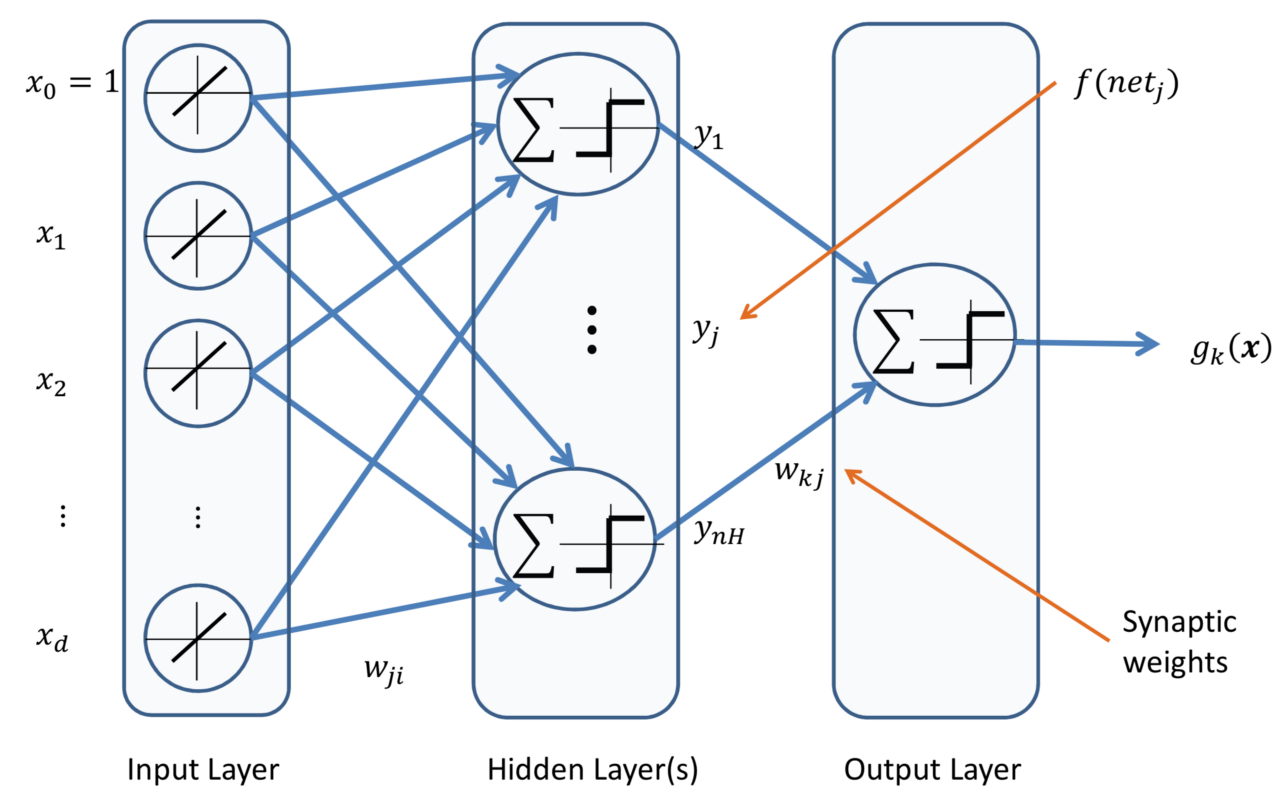
\includegraphics[width=0.6\linewidth]{images/introduction_neural.png}
	\caption{An artificial neuron with one input, one hidden and one output layer.}
	\label{fig:introduction_fig}
	\end{figure}

		\subsubsection{Towards Neural Nets}
A basic artificial neural network is a natural extension to perceptron. We can say that a basic neural network is a multi-layer perceptron called a feed-forward neural network.  An Artificial Neuron Network (ANN), popularly known as Neural Network is a computational model based on the structure and functions of biological neural networks. It is like an artificial human nervous system for receiving, processing, and transmitting information in terms of Computer Science. Basically, there are 3 different layers in a neural network, input layer, hidden layer and output layer. An ANN would contain :
		\begin{itemize}
			\item Hidden Layers
			\item Bias Units
			\item Neurons(input, output and perceptron)
			\item Synaptic weights
		\end{itemize}

	\subsection{Deep Neural Networks}
	Deep learning (also known as deep structured learning) is part of a broader family of machine learning methods based on artificial neural networks with representation learning. Learning can be supervised, semi-supervised or unsupervised.	\cite{bengio2013representation,schmidhuber2015deep}

Deep learning architectures such as deep neural networks, deep belief networks, recurrent neural networks and convolutional neural networks have been applied to fields including computer vision, speech recognition, natural language processing, audio recognition, social network filtering, machine translation, bioinformatics, drug design, medical image analysis, material inspection and board game programs, where they have produced results comparable to and in some cases surpassing human expert performance.\cite{krizhevsky2012imagenet}

Artificial neural networks (ANNs) were inspired by information processing and distributed communication nodes in biological systems. ANNs have various differences from biological brains. Specifically, neural networks tend to be static and symbolic, while the biological brain of most living organisms is dynamic (plastic) and analog.

\begin{figure}[htbp]
	\centering
		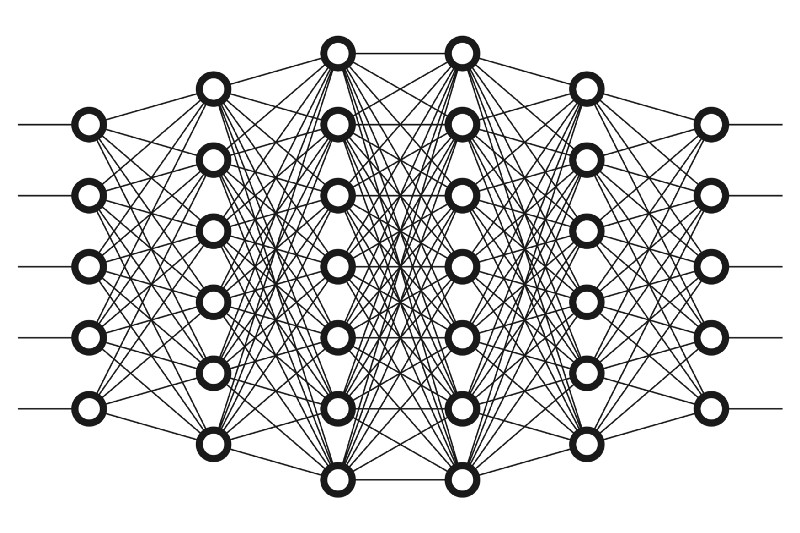
\includegraphics[width=0.6\linewidth]{images/deep_neural_network.jpeg}
	\caption{An deep neuron network with one input, four hidden and one output layer.}
	\label{fig:deep_neural_network}
	\end{figure}

Most modern deep learning models are based on artificial neural networks, specifically, Convolutional Neural Networks (CNN)s, although they can also include propositional formulas or latent variables organized layer-wise in deep generative models such as the nodes in deep belief networks and deep Boltzmann machines.\cite{bengio2009learning}

In deep learning, each level learns to transform its input data into a slightly more abstract and composite representation. In an image recognition application, the raw input may be a matrix of pixels; the first representational layer may abstract the pixels and encode edges; the second layer may compose and encode arrangements of edges; the third layer may encode a nose and eyes; and the fourth layer may recognize that the image contains a face. Importantly, a deep learning process can learn which features to optimally place in which level on its own. (Of course, this does not completely eliminate the need for hand-tuning; for example, varying numbers of layers and layer sizes can provide different degrees of abstraction.)\cite{bengio2013representation,lecun2015deep}


    \section{Learning Rule}

    Consider a trained three-layered (L-M-N) artificial neural network (ANN) of conventional neurons. The trained ANN consists of L number of input neurons, M number of hidden neurons, and N number of output neurons. The net potential of $m^{th}$ conventional hidden neuron is defined as 
    \begin{equation}
        V_m = \sum \limits_{l=1}^{L} w_{lm}x_{l} + w_{0m}x^{0}
    \end{equation}
    and its output is defined as 
    \begin{equation}
        Y_m = \quad f(V_m)
    \end{equation}
    Similarly, the net potential of $n^{th}$ output neuron is defined as
    \begin{equation}
        V_n = \sum \limits_{m=1}^{M} w_{mn}Y_{m} + w_{0n}x^{0}
    \end{equation}
    and its output is defined as 
    \begin{equation}
        Y_n = \quad f(V_n)
    \end{equation}

    Let $Y_n^D$ be the desired output and $Y_n^{Adv}$ be desired adversary output of the $n_{th}$ output neuron. Since the network's already trained, $Y_n^D - Y_n$ will be very small. Adversarial error due to output $(e_n^Y)$ can be calculated as $e_n^Y = Y_n^{Adv} - Y_n$. Adversary's goal is to generate a slightly perturbed version of $x^{Adv}$. To make small perturbations in the image, error $e^x$ is introduced. For $l_{th}$ input this error can be calculated as $e_l^x = x_l^{Adv} - x_l$. The cost function $(E)$ can be calculated using the mean square of both $e^Y$, and $e^x$ adversarial errors and expressed as
    \begin{equation}\label{eqn:error_function}
        E = \quad \frac{1}{2N} \sum \limits_{n=1}^{N} (e_n^Y)^{2} + \lambda \frac{1}{2L} \sum \limits_{l=1}^{L} (e_l^x)^{2}
    \end{equation}
    where, $\lambda$ is real number in range $(0,\infty)$ for target adversarial attack and for non-target adversarial attack, $\lambda = 0$. The goal is to keep reducing error $(E)$ by updating input $(x)$. The update rule adds the error gradient to input as 
    \begin{equation}\label{eqn:input_update_rule}
        x^{old} = x^{new} + \Delta x
    \end{equation} 
    For particular input $(x_l)$, $\Delta x_l$ can be calculated as
    \begin{equation}\label{eqn:delta_x_l}
        \Delta x_l= \frac{\eta}{N} \sum \limits_{m=0}^{M} \delta_{m} w_{lm} + \lambda \frac{\eta}{L} e_l^x
    \end{equation} 
    where, $$\delta_{m} = \left\{ \sum \limits_{n=0}^{N} \delta_{n} w_{mn} \right\} f'(V_m)$$, and $$\delta_{n} = e_n^Y f'(V_n)$$

    The \crefrange{eqn:error_function}{eqn:delta_x_l} is implemented as described in \crefrange{alg:forward_pass}{alg:update_weights}.


    
\SetKwInOut{Input}{input}
\SetKwInOut{Output}{output}

\begin{algorithm}[!h]
	\caption{Generate Adversarial Image}
	\label{alg:generate_image}
	\SetAlgoLined
	\Input{Desired input ($x^{Adv}$), Desired adversary output ($Y^{Adv}$), $\eta$, $\lambda$, Epochs }
	\Output{NULL}

	$x \leftarrow x^{Adv}$ \\
	\While{Epochs \textbf{is not} 0}{
		Forward-pass($x$) \\
		Backward-adversarial-pass($Y^{Adv}$)  \\
		Update-inputs($x, x^{Adv}, \eta, \lambda$)\\
		Epochs $\leftarrow$ Epochs $- 1$
	}
\end{algorithm}

\begin{algorithm}[!h]
	\caption{Forward-pass}
	\label{alg:forward_pass}
	\SetAlgoLined
	\Input{Input Vector ($x$)}
	\Output{Predicted Output Vector ($y$)}
	\For{ i $\leftarrow  0$ \KwTo num\_layers $-1$  }{
		\ForEach {neuron, m \textbf{in} $layer_{i}$} {
			$V_m^{i} \leftarrow \displaystyle{\sum \limits_{l=1}^{len(x)} w_{lm}x_{l} + w_{0m}x^{0}}$ \\
			$Y_m^{i} \leftarrow f(V_m^{i})$		
		}
		$x \leftarrow Y^{i}$\\
	}  
\end{algorithm}

\begin{algorithm}[!h]
	\caption{Backward-adversarial-pass}
	\label{alg:backward_pass}
	\SetAlgoLined
	\Input{Predicted Output Vector ($y$)}
	\Output{NULL}
	\For{ i $\leftarrow$ num\_layers $-1$ \KwTo $0$  }{
		\If {$layer_{i}$ \textbf{is} Output-Layer}{
			\ForEach {neuron, n \textbf{in} $layer_{i}$} {
				$\Delta_{n}^{i} \leftarrow \Big\{ e_n^{i} \cdot f'(V_n^{i}) \Big\} $\\
			}
		}
		\Else{
			\ForEach { neuron, m \textbf{in} $layer_{i}$} {
				$e_m^{i}  \leftarrow 0$ \\
				\ForEach {neuron, n \textbf{in} $layer_{i+1}$} {
					$e_m^{i} \leftarrow e_m^{i} + \Big\{ w_{mn} \cdot \Delta_{n}^{i+1}   \Big\} $ \\
				}			
				$\Delta_{m}^{i} \leftarrow \Big\{ e_m^{i} \cdot f'(V_m^{i}) \Big\} $\\

			} 	
		} 
	}  
\end{algorithm}


\begin{algorithm}[!h]
	\caption{Update-inputs}
	\label{alg:update_weights}
	\SetAlgoLined
	\Input{Input Vector ($x$), Desired input ($x^D$), $\eta$, $\lambda$}
	\Output{NULL}	
		\For{ i $\leftarrow 0$ \KwTo $len(x) - 1$} {
				$x_i \leftarrow x^i + \dfrac{\eta}{N} \left\{ \Delta_{i}^{0}  + \lambda \cdot (x_i^D - x_i) \right\} $\\
				\tcp*[f]{N is the number of output neurons}
				$x_i \leftarrow x^i + \eta \left\{ \dfrac{1}{N} \Delta_{i}^{0}  + \dfrac{\lambda}{L} \cdot (x_i^D - x_i) \right\} $\\

		}				
\end{algorithm}


    \section{Performance Evaluation}
    \subsection*{Training ANN}
        
        An ANN with structure $[784-20-10]$ with sigmoid activation function is constructed and compiled with stochastic gradient descent (SGD) as optimizer and mean square error (MSE) as loss function. The network consists of one hidden layer with $20$ neurons and one output layer with $10$ neurons. 

        The compiled network is trained on a subset of MNIST dataset consisting of random $600$ training samples and $100$ testing samples. The network was able to achieve training accuracy of $96\%$ and testing accuracy of $89\%$. \Cref{fig:training_results} illustrates testing performance of trained network.

        \begin{figure}[H]
            \centering
            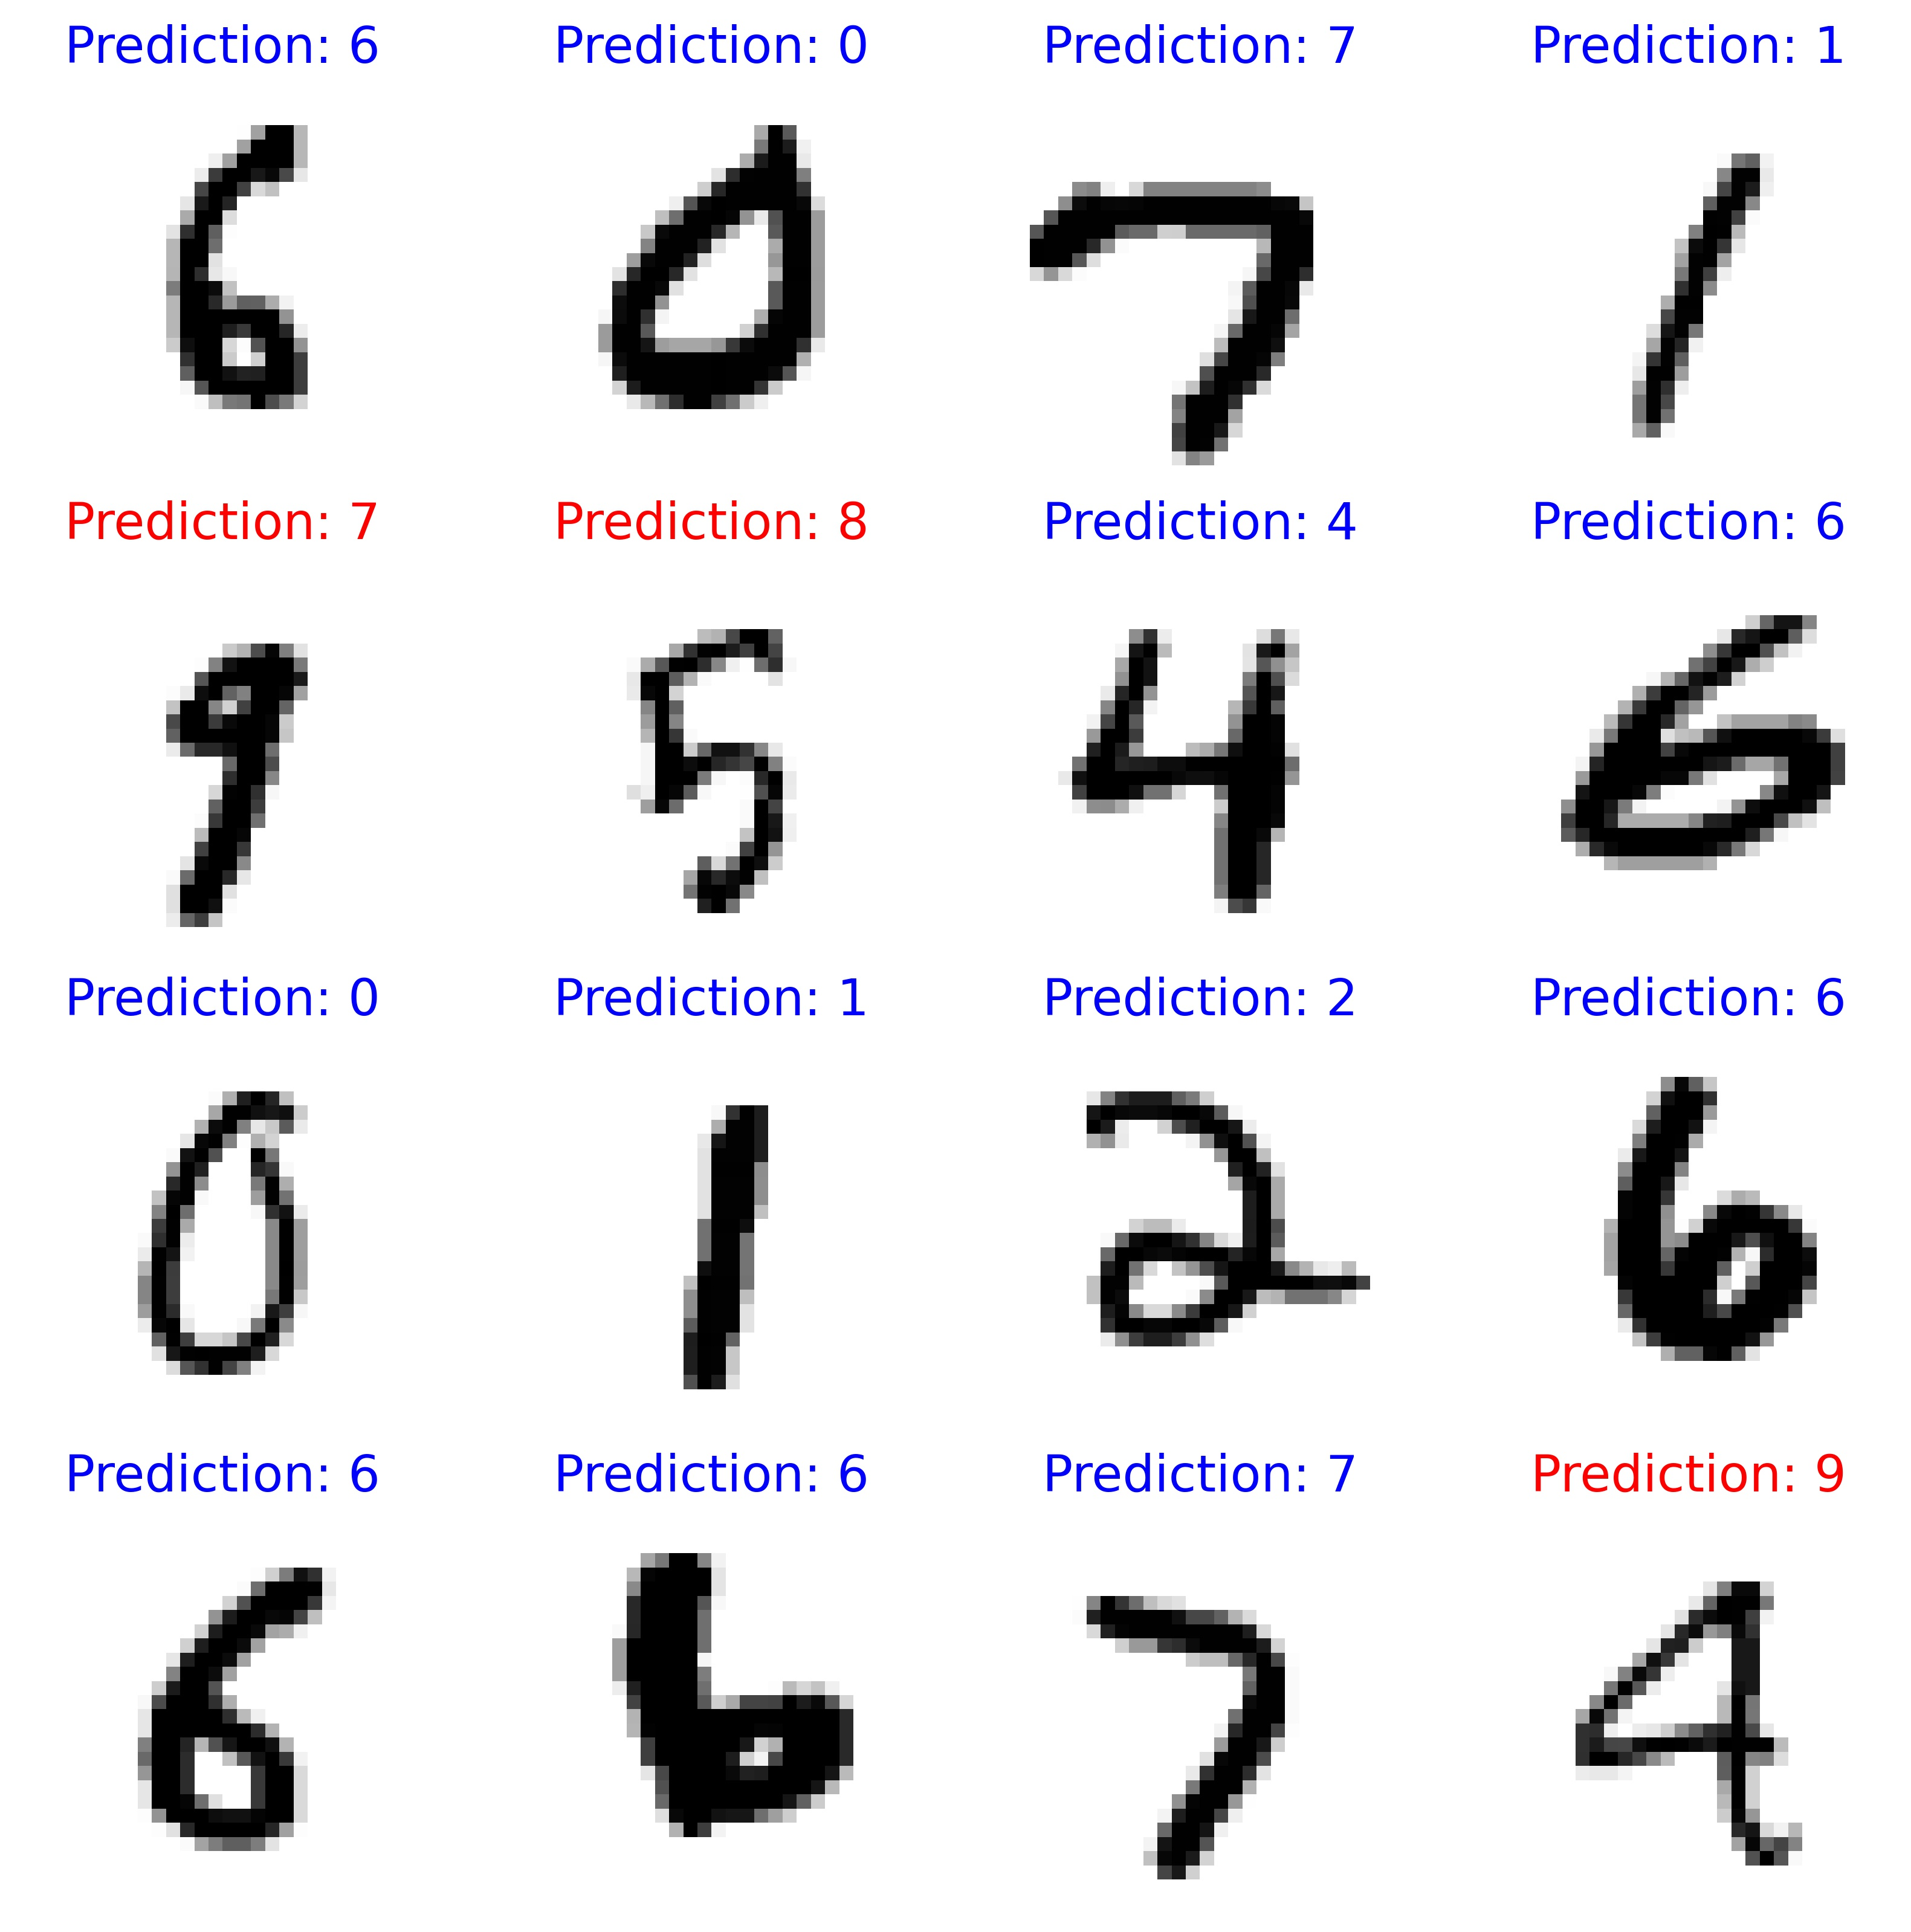
\includegraphics[width=\linewidth]{images/trained_predictions.jpg}
            \caption{Predictions of trained network on test set}
            \label{fig:training_results}
        \end{figure}

    \subsection*{Target Adversarial Attack}

        For generating adversarial images, \crefrange{alg:generate_image}{alg:update_weights} are used where  adversary just need to pass target image $(x^{Adv})$ and goal $(Y^{Adv})$ in \cref{alg:generate_image}. For generating adversarial images $\lambda = 0.8$ is considered. A noise will be generated as an adversarial image if $\lambda = 0$ is considered. \Cref{fig:adversarial_images} consists of all generated adversarial images using which target adversarial attack was successful. In \cref{fig:adversarial_images} it can also be observed how prediction confidence changed when adversarial image is used. Some generated images as shown in \cref{fig:adversarial_images_unsuccessful} were not able to fool the trained network, but it is worth to notice that network confidence in correctly predicting particular image is decreased, so they can be termed as incomplete attacks.    

        \begin{figure}[H]
            \centering
            \begin{subfigure}{0.7\linewidth}
                \centering
                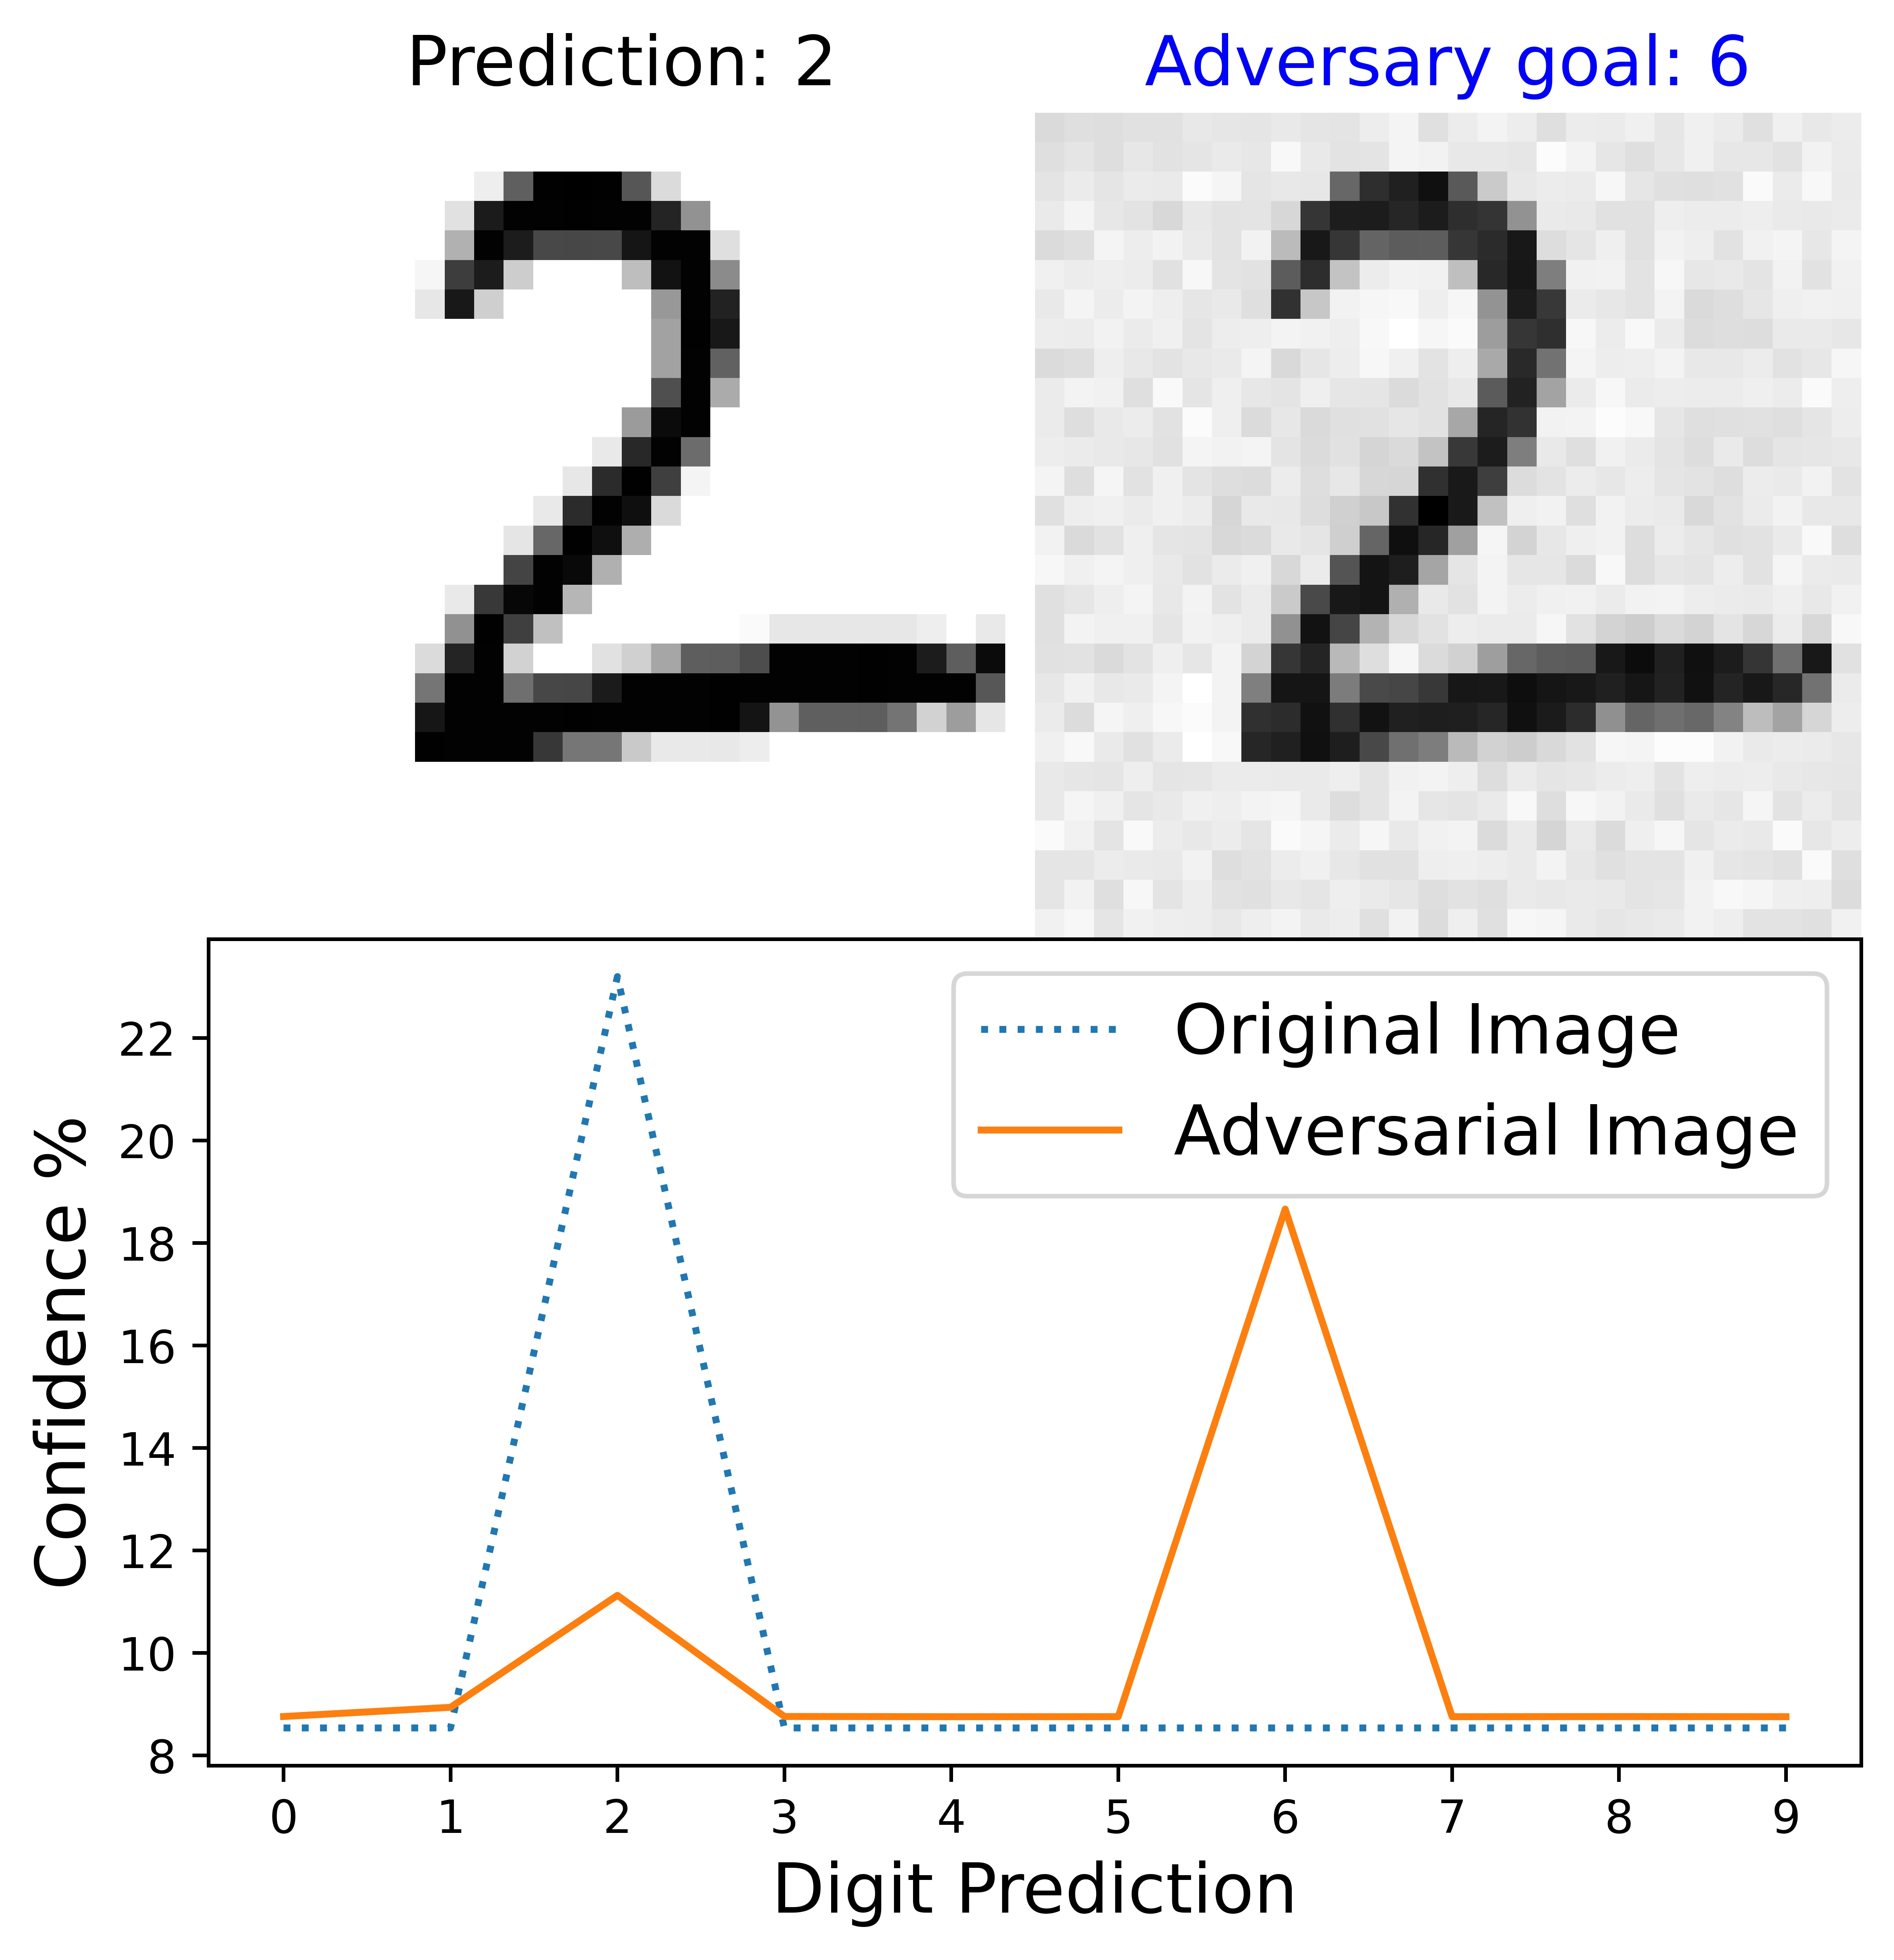
\includegraphics[width=\textwidth]{images/generated_adversarial_image_3.jpg}
                \caption{}
            \end{subfigure}
            % \begin{subfigure}{0.7\linewidth}
            %     \centering
            %     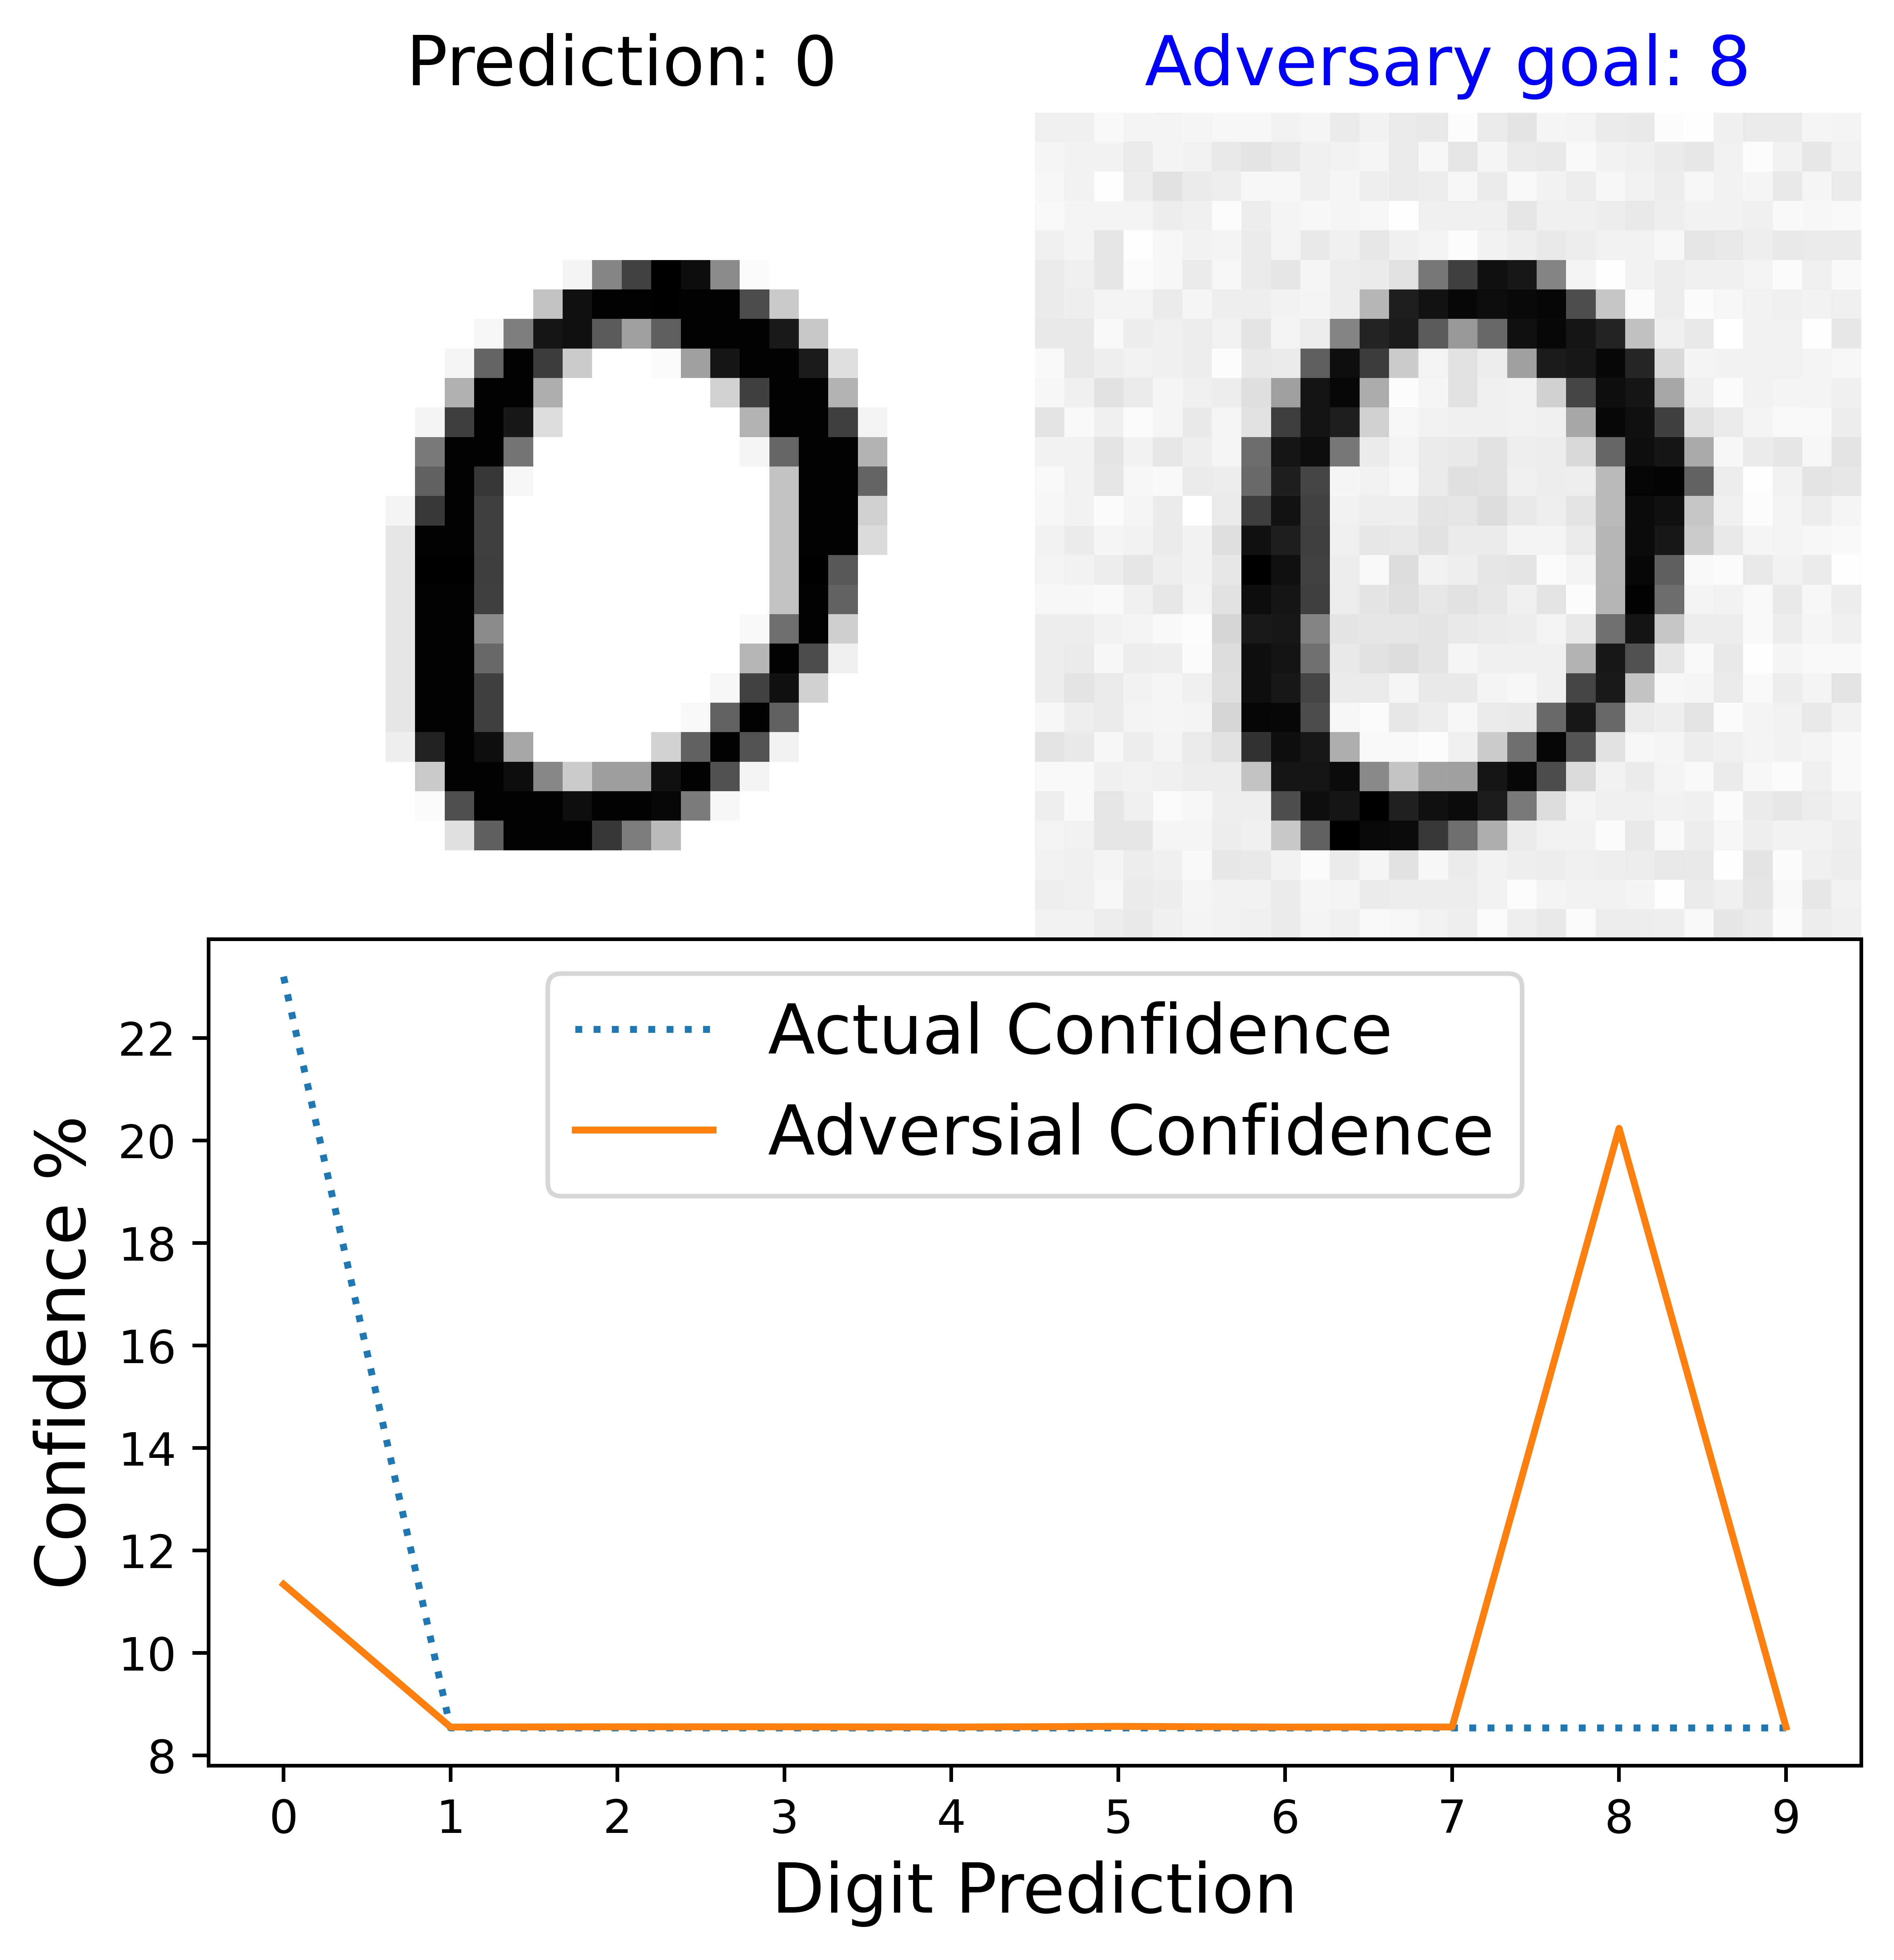
\includegraphics[width=\textwidth]{images/generated_adversarial_image_2.jpg}
            %     \caption{}
            % \end{subfigure}
            \begin{subfigure}{0.7\linewidth}
                \centering
                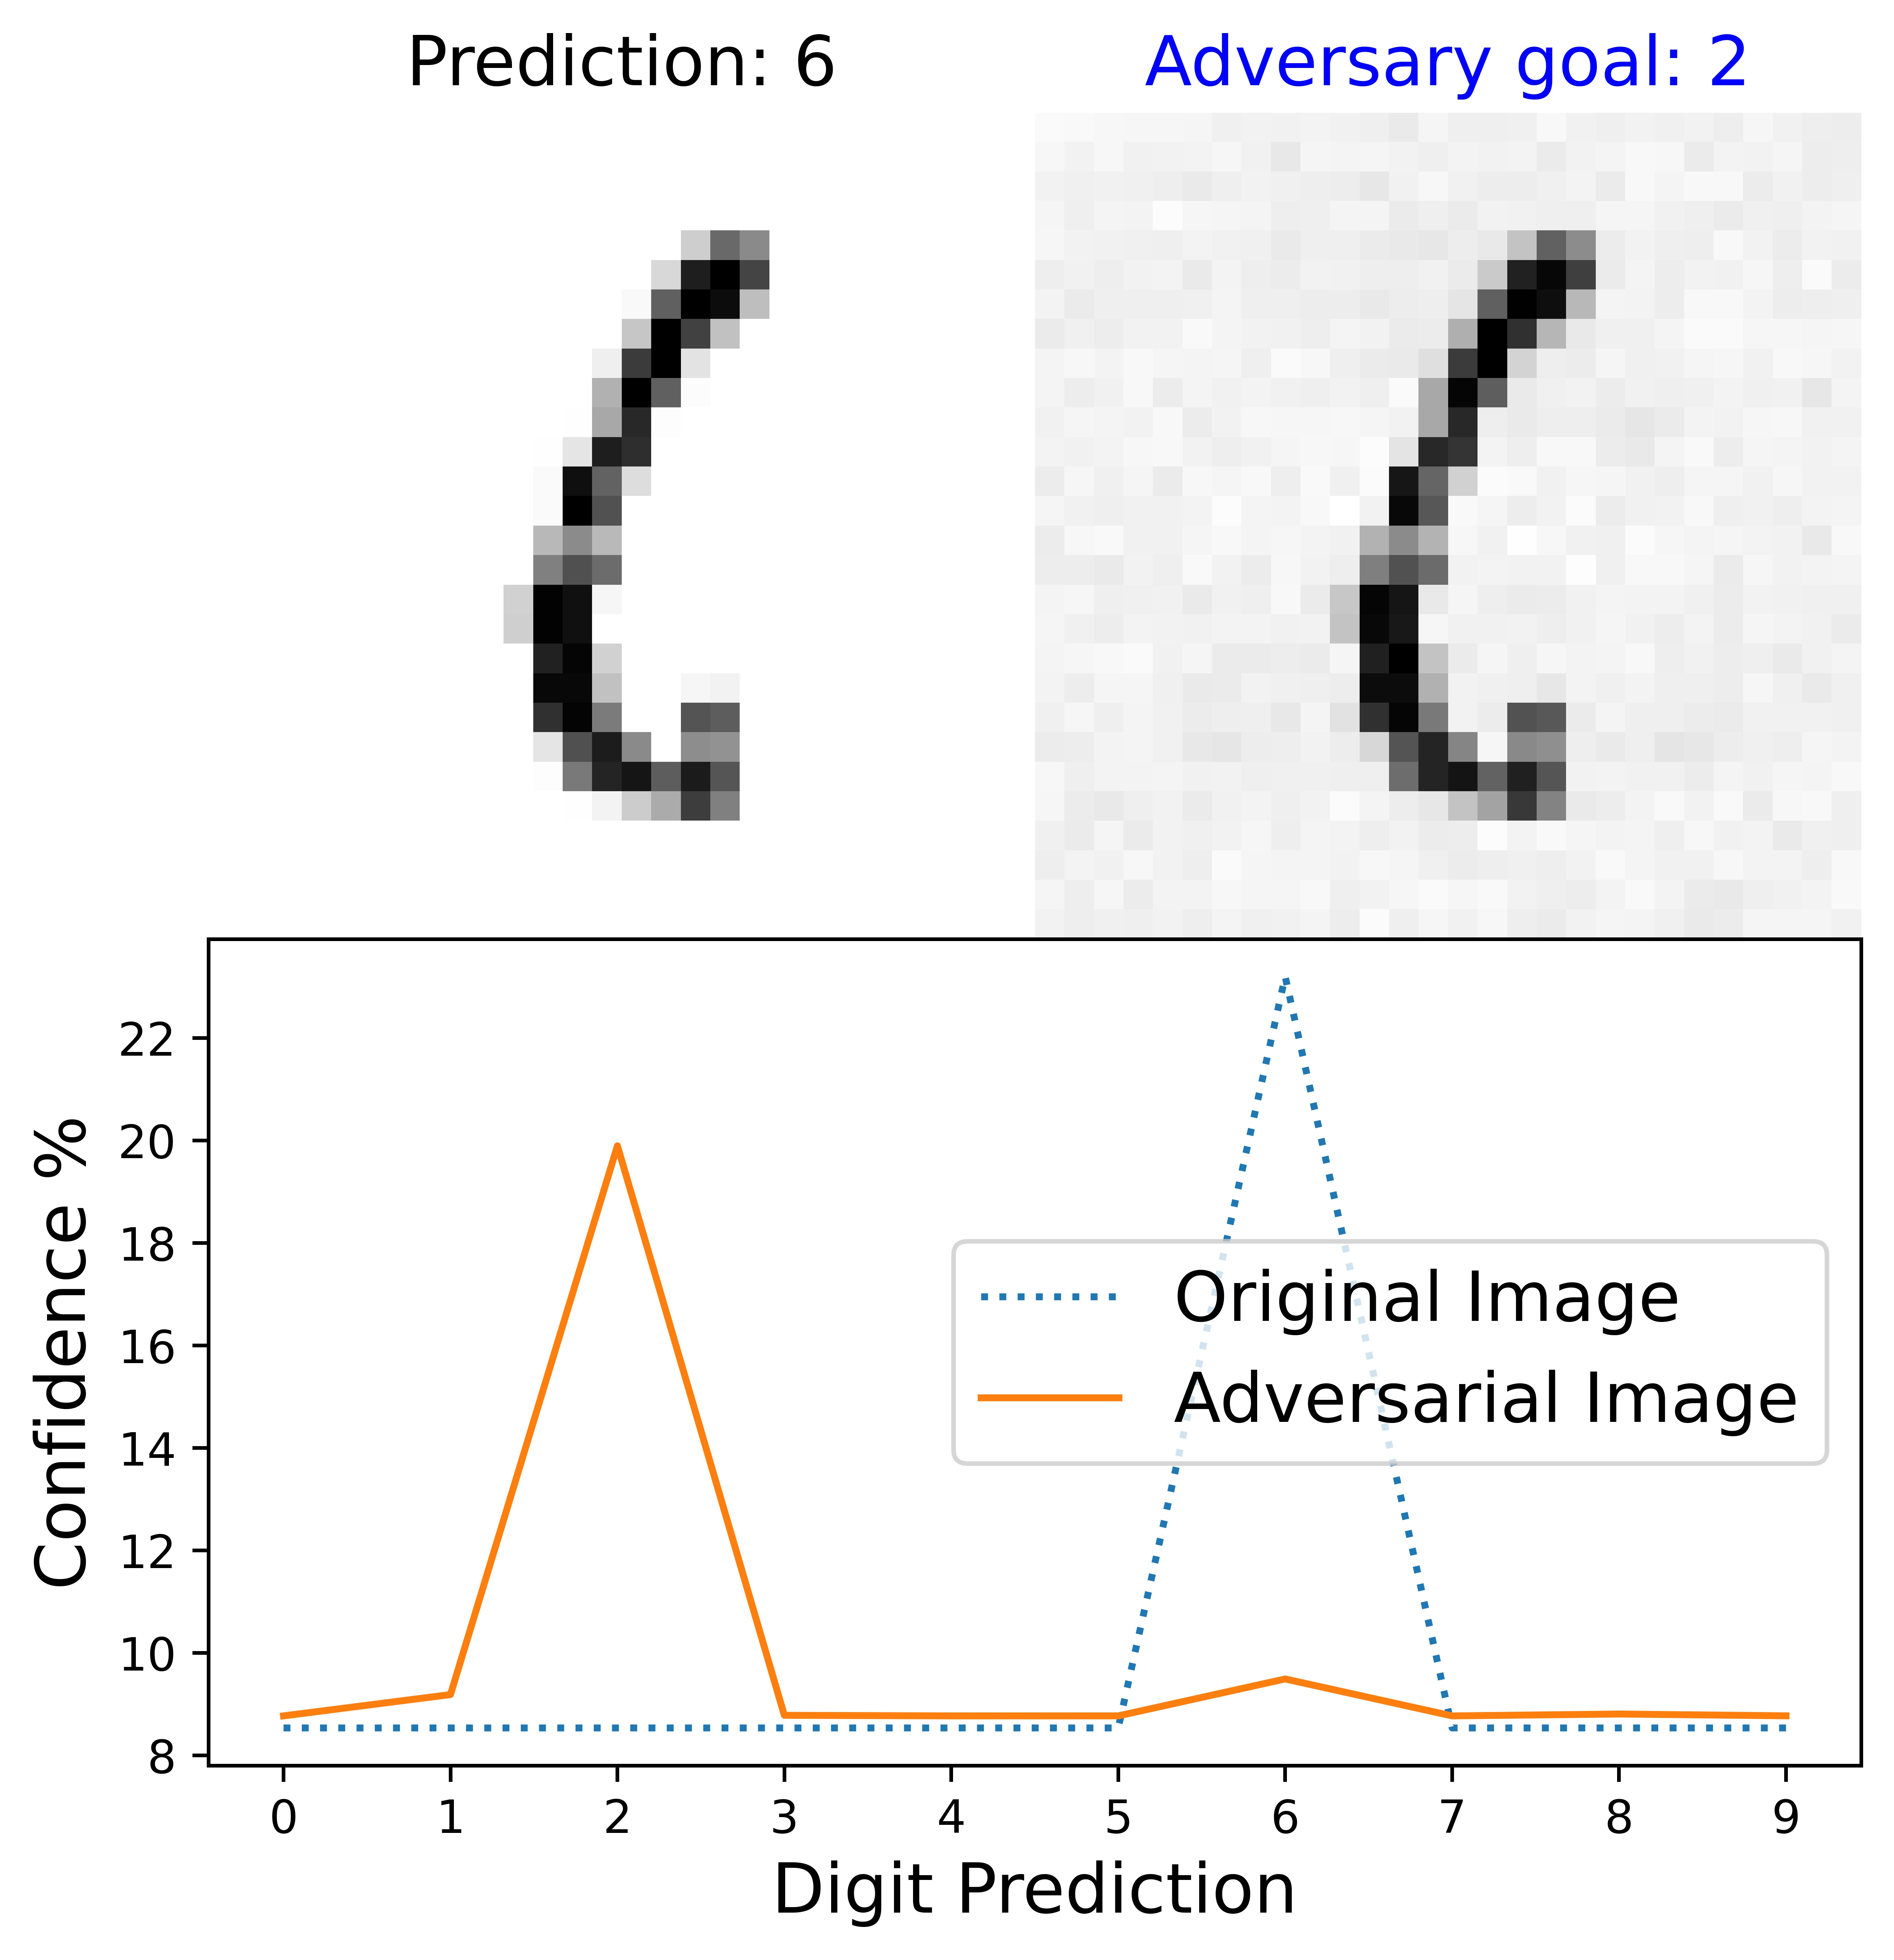
\includegraphics[width=\textwidth]{images/generated_adversarial_image_4.jpg}
                \caption{}
            \end{subfigure}
            \caption{Some original images (in left) and generated adversarial images (in right) with their prediction (below)}
            \label{fig:adversarial_images}
        \end{figure}

        % \begin{figure}[htbp]
        %     \centering
        %     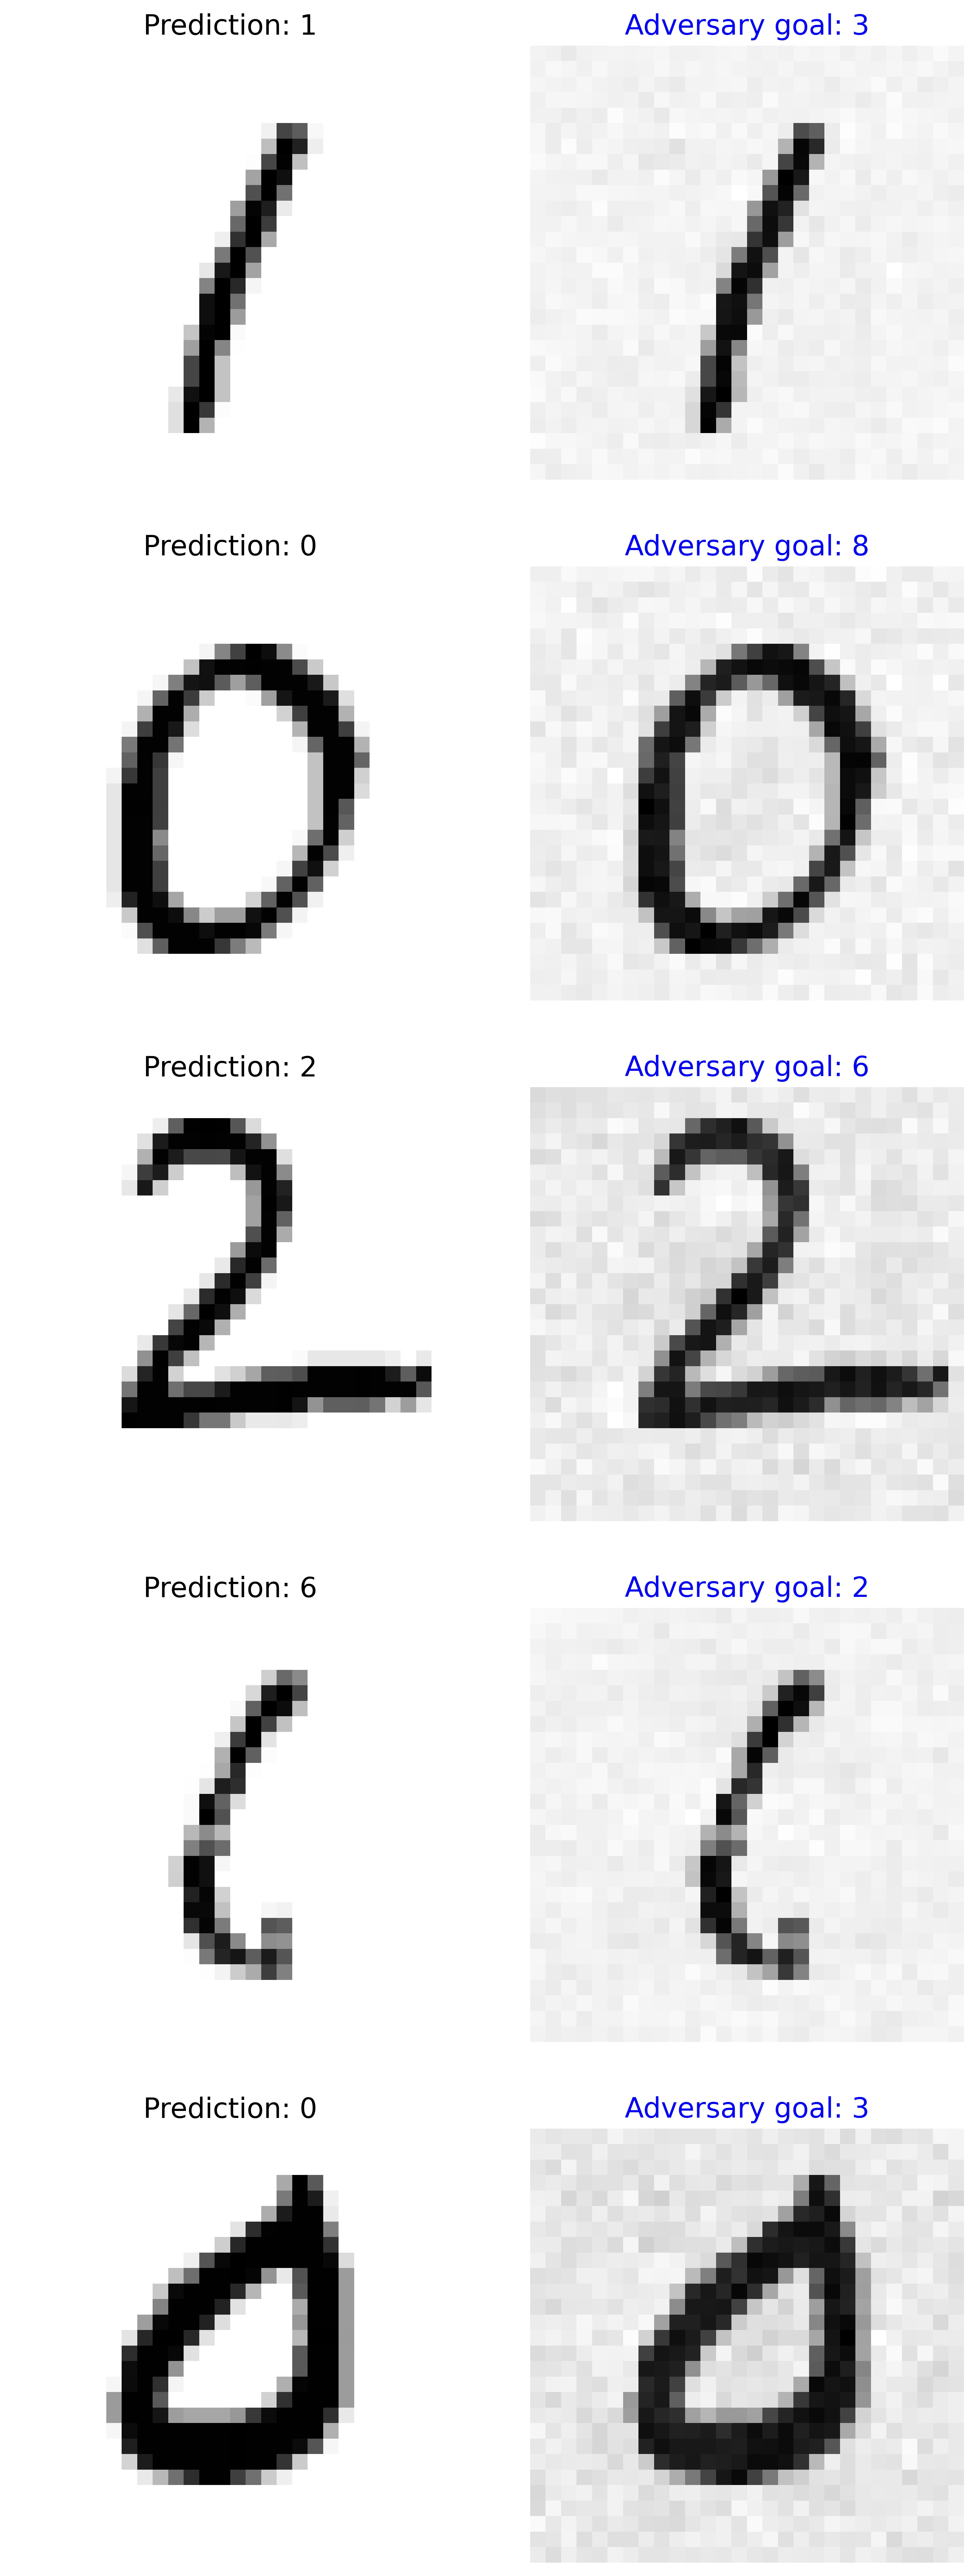
\includegraphics[width=\linewidth]{images/generated_adversarial_images.jpg}
        %     \caption{Some target adversarial images (in left) and generated adversarial images (in right) with adversary goal and actual prediction}
        %     \label{fig:adversarial_images}
        % \end{figure}

        \begin{figure}[!h]
            \centering
            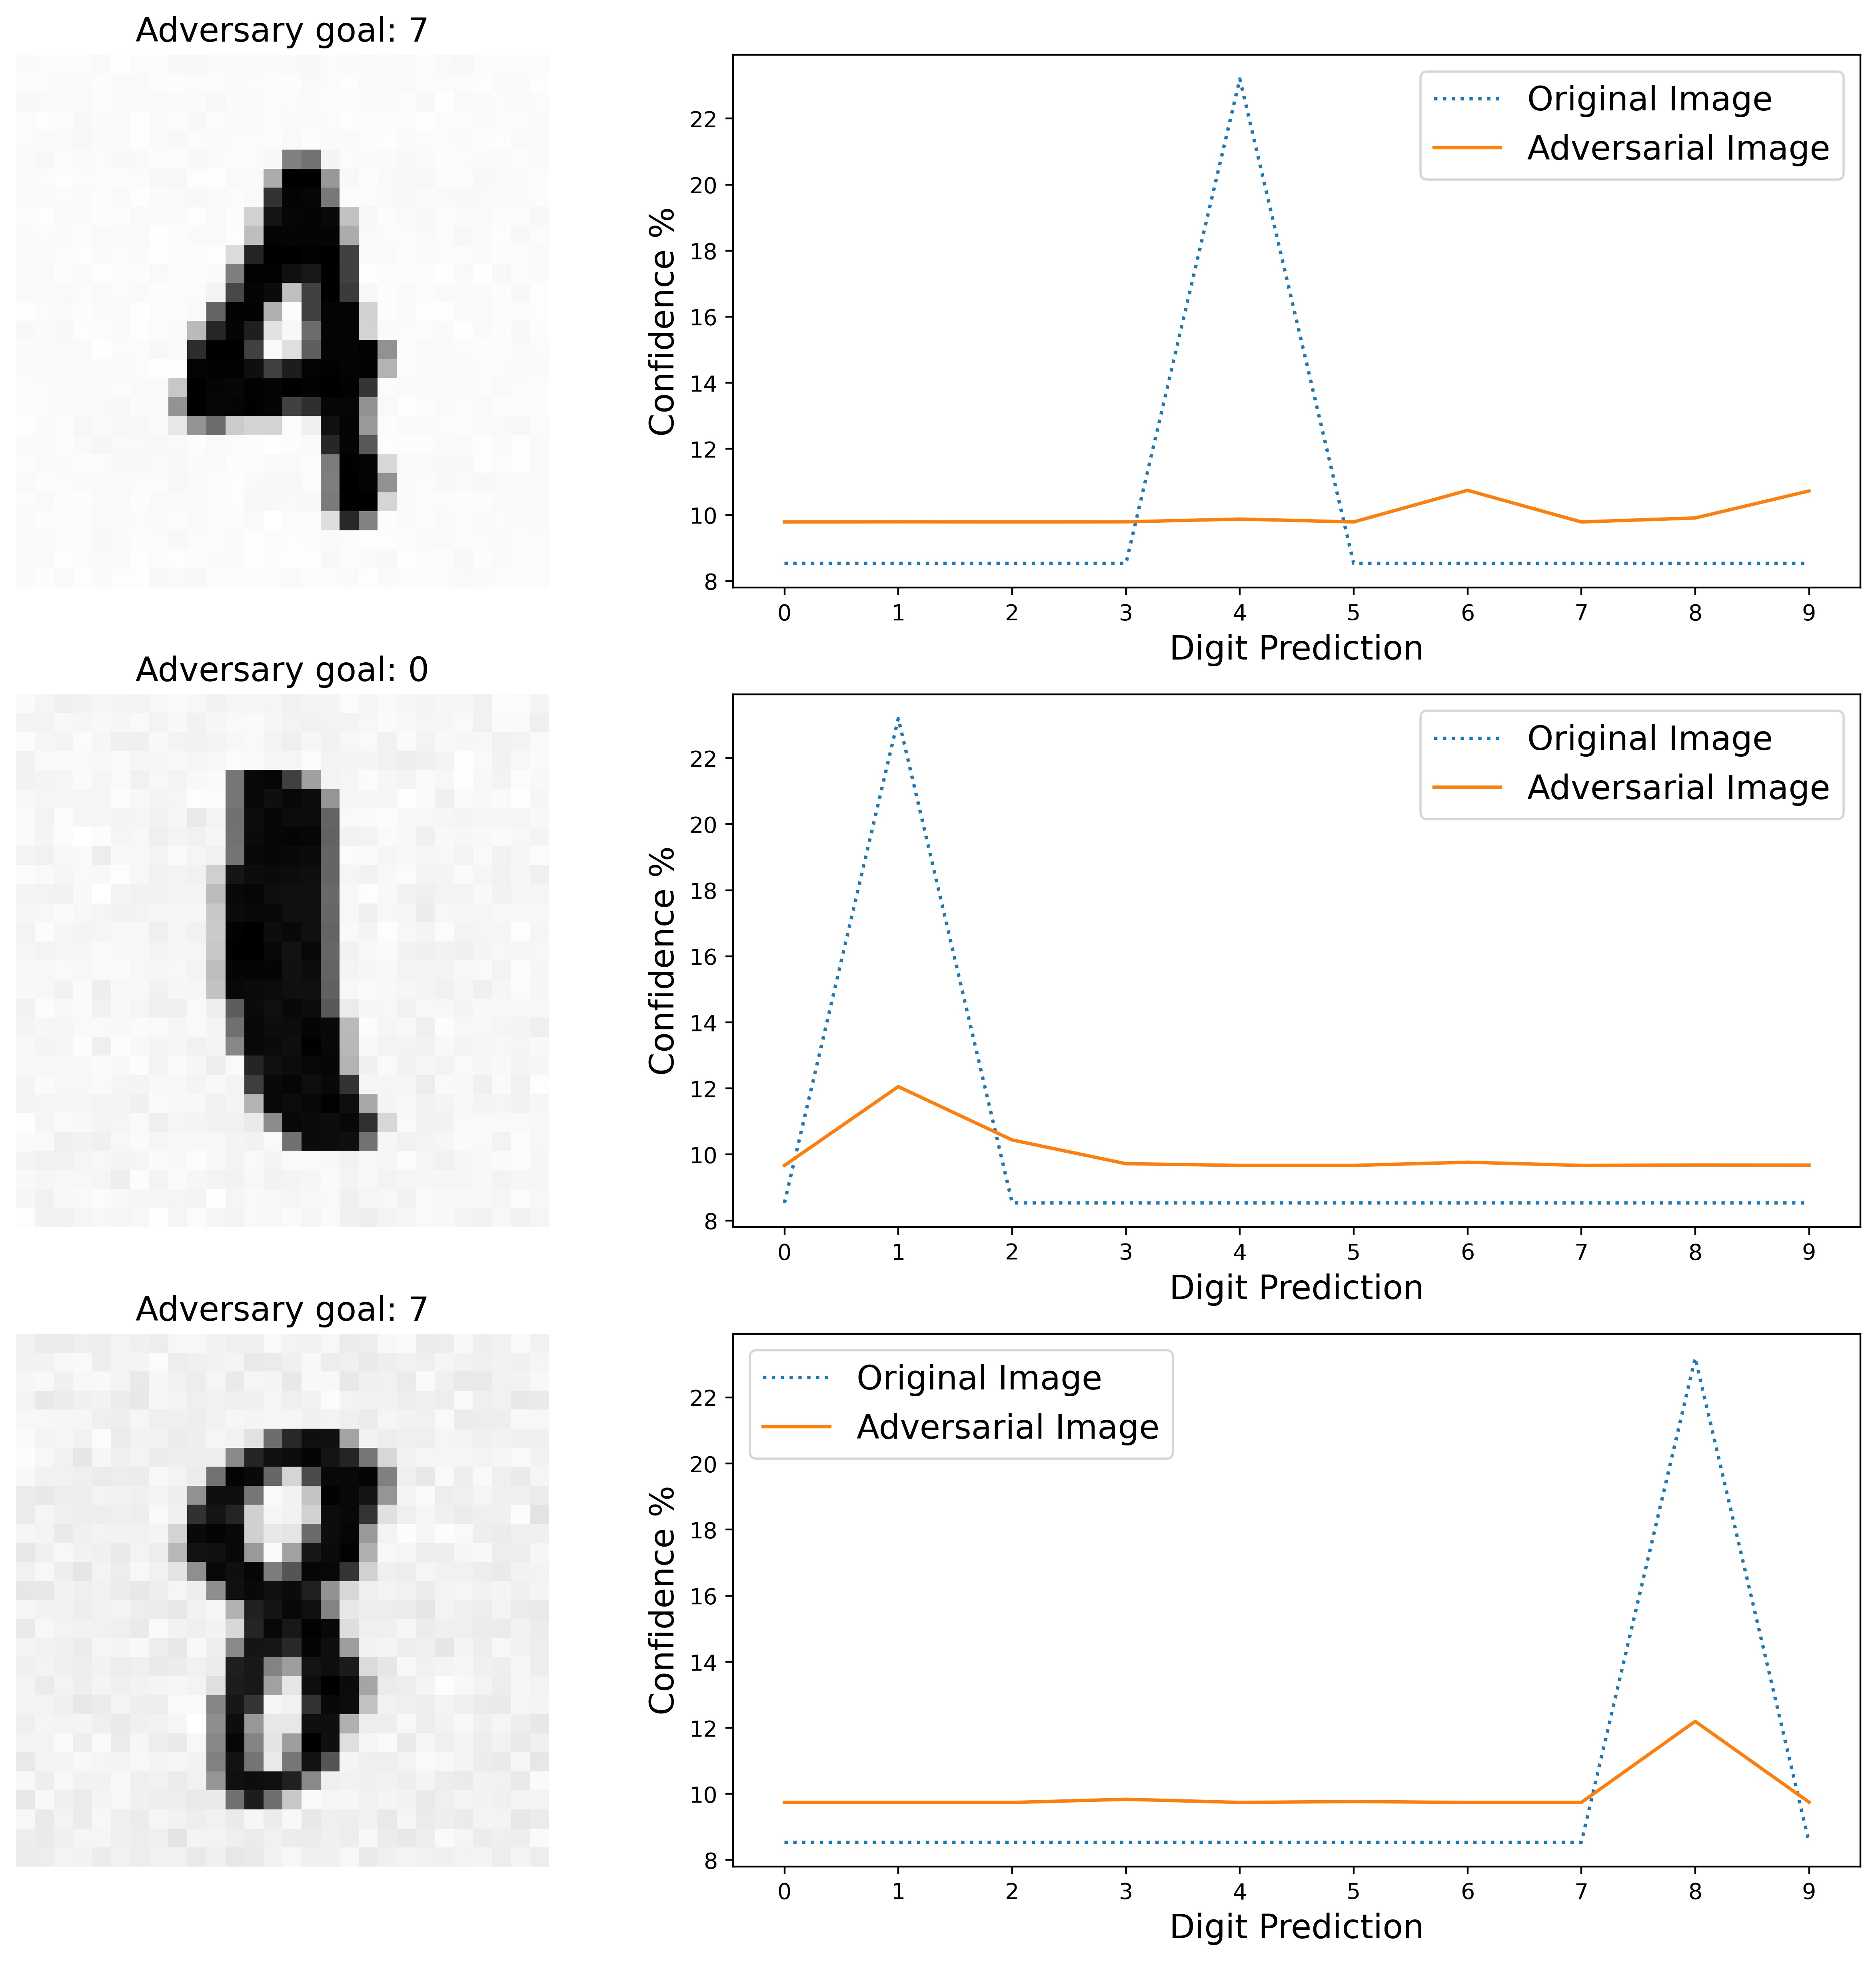
\includegraphics[width=\linewidth]{images/generated_adversarial_images_unsuccessful.jpg}
            \caption{Some generated adversarial images (in left) using which attack was not successful with its prediction (in right)}
            \label{fig:adversarial_images_unsuccessful}
        \end{figure}

    

    % \section{Adversarial machine learning}
	
	Adversarial machine learning is a technique employed in the field of machine learning which attempts to fool models through malicious input. This technique can be applied for a variety of reasons, the most common being to attack or cause a malfunction in standard machine learning models.

Machine learning techniques were originally designed for stationary and benign environments in which the training and test data are assumed to be generated from the same statistical distribution. However, when those models are implemented in the real world, the presence of intelligent and adaptive adversaries may violate that statistical assumption to some degree, depending on the adversary. This technique shows how a malicious adversary can surreptitiously manipulate the input data so as to exploit specific vulnerabilities of learning algorithms and compromise the security of the machine learning system.\cite{lim2019algorithmic,goodfellow2018making}

		\section{History}
		As early as Snow Crash (1992), science fiction writers have posited scenarios of technology being vulnerable to specially-constructed data. In Zero History (2010), a character dons a t-shirt decorated in a way that renders him invisible to electronic surveillance.\cite{vincent2017magic}

In 2004, Nilesh Dalvi and others noted that linear classifiers used in spam filters were being defeated by simple "evasion attacks" as spammers inserted "good words" into their spam emails. (Around 2007, some spammers would also add random noise to fuzz words within "image spam" in order to defeat OCR-based filters.) In 2006, Marco Barreno and others published "Can Machine Learning Be Secure?", an influential paper suggesting a broad taxonomy of attacks against machine learning. As late as 2013 many researchers continued to hope that non-linear classifiers (such as SVMs and neural networks) might be naturally robust to adversarial examples. In 2012, deep neural networks were unexpectedly crowned as the dominant path for advanced computer vision; starting in 2014, Christian Szegedy and others demonstrated that deep neural networks could be fooled with tiny adjustments of the input.\cite{biggio2018wild}


While it is known that neural networks are vulnerable to small perturbations to inputs that dramatically change a network's output, the most popular setting for studying these adversarial attacks to date is image classification. Adversarial attacks in this domain perturb an image to fool a classifier while constraining the perturbation to be small in some norm. While classical adversarial perturbations are designed for a single image, “universal” perturbations are crafted to fool the classifier when applied to nearly any image . Similar attacks exist for other vision tasks like detection and segmentation. Other domains, such as natural language and graph structured data, have attracted the attention of adversarial attacks, but these attacks are impractical. For example, in NLP, adversarial text may be nonsensical, and in graph structured data, attackers are weak.


    % \section{Definitions and Notations}
    In this section, a brief introduction to the key components of model attacks and defences is presented. I  hope that my explanations can help audience to understand the main components of the related works on adversarial attacks and their countermeasures. By answering the following questions, we define the main terminology:

    \begin{itemize}
        \item \textit{Adversary's Goal} 

        What is the goal or purpose of the attacker? Does he want to misguide the classifier's decision on one sample, or influence the overall performance of the classifier?
        \item \textit{Adversary's Knowledge}

        What information is available to the attacker? Does he know the classifier's structure, its parameters or the training set used for classifier training?
        \item \textit{Victim Models}

        What kind of deep learning models do adversaries usually attack? Why are adversaries interested in attacking these models?
        \item \textit{Security Evaluation}

        How can we evaluate the safety of a victim model when faced with adversarial examples? What is the relationship and difference between these security metrics and other model goodness metrics, such as accuracy or risks?
    \end{itemize}

	\section{Threat Model}
		\subsection{Adversary's Goal}
		\begin{itemize}
		\item \textit{Poisoning Attack vs Evasion Attack}
		
		Poisoning attacks refer to the attacking algorithms that allow an attacker to insert/modify several fake samples into the training database of a DNN algorithm. These fake samples can cause failures of the trained classifier. They can result in the poor accuracy, or wrong prediction on some given test samples. This type of attacks frequently appears in the situation where the adversary has access to the training database. For example, web-based repositories and “honeypots” often collect malware examples for training, which provides an opportunity for adversaries to poison the data.
		
		In evasion attacks, the classifiers are fixed and usually have good performance on benign testing samples. The adversaries do not have authority to change the classifier or its parameters, but they craft some fake samples that the classifier cannot recognize. In other words, the adversaries generate some fraudulent examples to evade detection by the classifier. For example, in autonomous driving vehicles, sticking a few pieces of tapes on the stop signs can confuse the vehicle's road
sign recognizer.		

			\item \textit{Targeted Attack vs Non-Targeted Attack}
			
			In targeted attack, when the victim sample $(x, y)$ is given, where $x$ is feature vector and $y \in Y$ is the ground truth label of $x$, the adversary aims to induce the classifier to give a specific label $t \in Y$ to the perturbed sample $x'$. For example, a fraudster is likely to attack a financial company's credit evaluation model to disguise himself as a highly credible client of this company.

If there is no specified target label $t$ for the victim sample $x$, the attack is called non-targeted attack. The adversary only wants the classifier to predict incorrectly.
		\end{itemize}

		\subsection{Adversary's Knowledge}		
            \begin{itemize}
                \item \textit{White-Box Attack}
                
                In a white-box setting, the adversary has access to all the information of the target neural network, including its architecture, parameters, gradients, etc. The adversary can make full use of the network information to carefully craft adversarial examples. White-box attacks have been extensively studied because the disclosure of model architecture and parameters helps people understand the weakness of DNN models clearly and it can be analysed mathematically. Security against white-box attacks is the property that we desire ML models to have.
            
                \item \textit{Black-Box Attack}
                In a black-box attack setting, the inner configuration of DNN models is unavailable to adversaries. Adversaries can only feed the input data and query the outputs of the models. They usually attack the models by keeping feeding samples to the box and observing the output to exploit the model's input-output relationship, and identity its weakness. Compared to white-box attacks, black-box attacks are more practical in applications because model designers usually do not open source their model parameters for proprietary reasons.	
            
                \item \textit{Semi-white (Gray) Box Attack}	
                
                In a semi-white box or gray box attack setting, the attacker trains a generative model for producing adversarial examples in a white-box setting. Once the generative model is trained, the attacker does not need victim model any more, and can craft adversarial examples in a black-box setting.
            \end{itemize}
            
		\subsection{Victim Models}
    		Following machine learning models are susceptible to adversarial examples, and some popular deep learning architectures used in image, graph and text data domains.
		
            \begin{enumerate}
                \item \textbf{Conventional Machine Learning Models}
                
                For conventional machine learning tools, there is a long history of studying safety issues. Some researchers have attacked SVM classifiers and fully-connected shallow neural networks for the MNIST dataset. Some of them examined the security of SpamBayes, a Bayesian method based spam detection software. The security of Naive Bayes classifiers is also checked. Many of these ideas and strategies have been adopted in the study of adversarial attacks in deep neural networks.
                \item \textbf{Deep Neural Networks}
                
                Different from traditional machine learning techniques which require domain knowledge and manual feature engineering, DNNs are end-to-end learning algorithms. The models use raw data directly as input to the model, and learn objects underlying structures and attributes. The end-to-end architecture of DNNs makes it easy for adversaries to exploit their weakness, and generate high-quality deceptive inputs (adversarial examples). Moreover, because of the implicit nature of DNNs, some of their properties are still not well understood or interpretable. Therefore, studying the security issues of DNN models is necessary. Next, I have briefly introduced some of popular victim deep learning models which are used as “benchmark” models in attack/defence studies.
                    \begin{itemize}
                        \item \textit{Fully-Connected Neural Networks}
                        
                        Fully-connected neural networks (FC) are composed of layers of artificial neurons. In each layer, the neurons take the input from previous layers, process it with the activation function and send it to the next layer; the input of first layer is sample $x$, and the (softmax) output of last layer is the score $F(x)$.
                        \item \textit{Convolutional Neural Networks}		
                        
                        In computer vision tasks, Convolutional Neural Networks is one of the most widely used models. CNN models aggregate the local features from the image to learn the representations of image objects. CNN models can be viewed as a sparse-version of fully connected neural networks: most of the weights between layers are zero. Its training algorithm or gradients calculation can also be inherited from fully connected neural networks.
                        \item \textit{Graph Convolutional Networks}
                        
                        The graph convolutional networks later became a popular node classification model for graph data. The idea of graph convolutional networks is similar to CNN. It aggregates the information from neighbour nodes to learn representations for each node $v$, and outputs the score $F(v,X)$ for prediction.
                        
                        \item \textit{Recurrent Neural Networks}
                        
                        Recurrent Neural Networks are very useful for tackling sequential data. As a result, they are widely used in natural language processing. The RNN models, especially LSTM are able to store the previous time information in memory, and exploit useful information from previous sequence for next-step prediction.
                    \end{itemize}
            \end{enumerate}


    % \section{Some Adversarial Attacks}		
	In this section we will see some of the adversarial attacks done by some researchers on novel machine learning models and deep learning architectures. These attacks raises a serious and important question, Is it really safe to use neural networks and continue to invest in them? Let's see some of the examples now.
	
	\begin{enumerate}
        \item  In 2014, a group of researchers at Google and NYU found that it was far too easy to fool ConvNets with an imperceivable, but carefully constructed nudge in the input. Let’s look at an example. We start with an image of a panda, which our neural network correctly recognizes as a “panda” with $57.7 \%$ confidence. Add a little bit of carefully constructed noise and the same neural network now thinks this is an image of a gibbon with $99.3 \%$ confidence! This is, clearly, an optical illusion — but for the neural network. You and I can clearly tell that both the images look like pandas — in fact, we can’t even tell that some noise has been added to the original image to construct the adversarial example on the right! \Cref{fig:panda_attack} represents the the actual and adversarial image.
            \begin{figure}[htbp]
                \centering
                    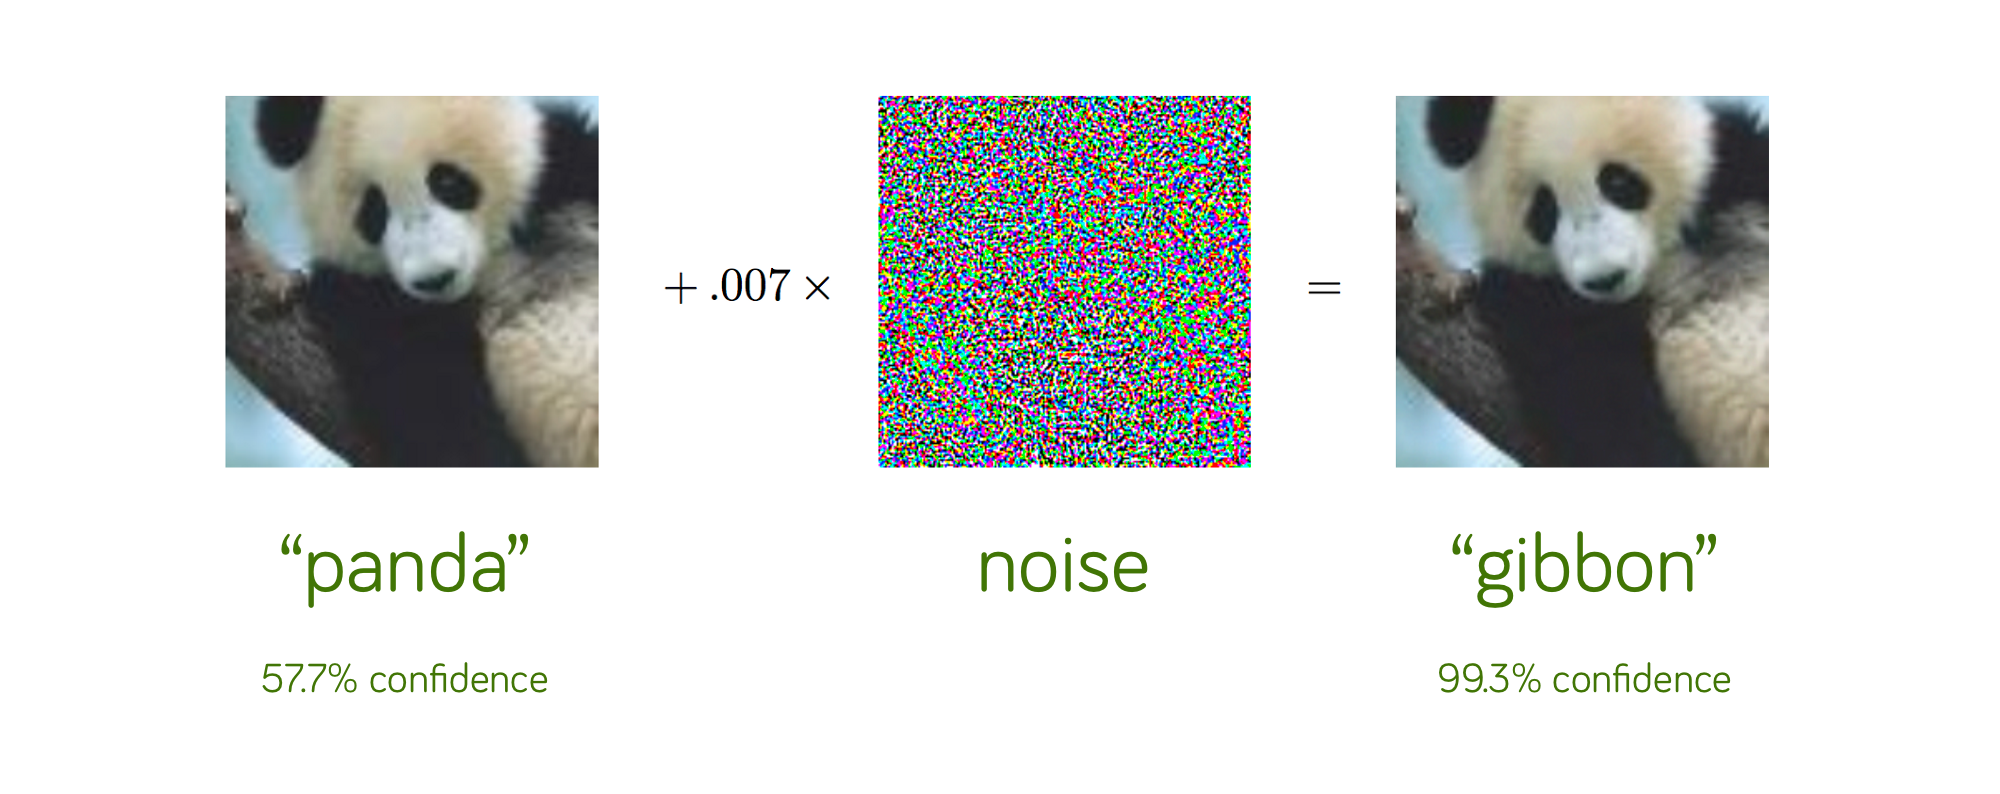
\includegraphics[width=0.8\linewidth]{images/panda_attack.png}
                \caption{An actual image of panda with a perturbation makes a novel deep neural network to misclassify as gibbon.}
                \label{fig:panda_attack}
            \end{figure}

        \item In 2017, another group demonstrated that it’s possible for these adversarial examples to generalize to the real world by showing that when printed out, an adversarially constructed image will continue to fool neural networks under different lighting and orientations. \Cref	{fig:example1} shows that an adversarial image  can be printed and any novel model will still misclassify it.
        
            \begin{figure}[htbp]
                \centering
                    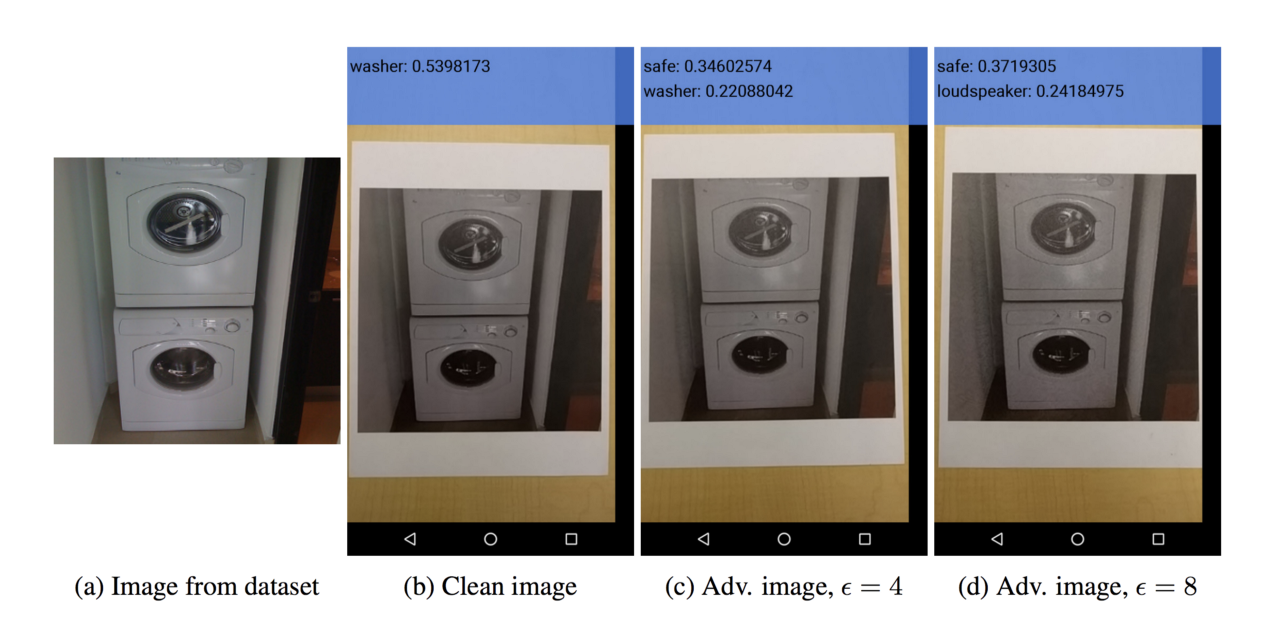
\includegraphics[width=0.7\linewidth]{images/example1.png}
                \caption{Printed adversarial image}
                \label{fig:example1}
            \end{figure}	
        \item Another interesting work, titled “Accessorize to a Crime: Real and Stealthy Attacks on State-of-the-Art Face Recognition” showed that one can fool facial recognition software by constructing adversarial glasses by dodging face detection altogether. The glasses in \cref{fig:example2} could let anyone impersonate someone else as well

            \begin{figure}[htbp]
                \centering
                    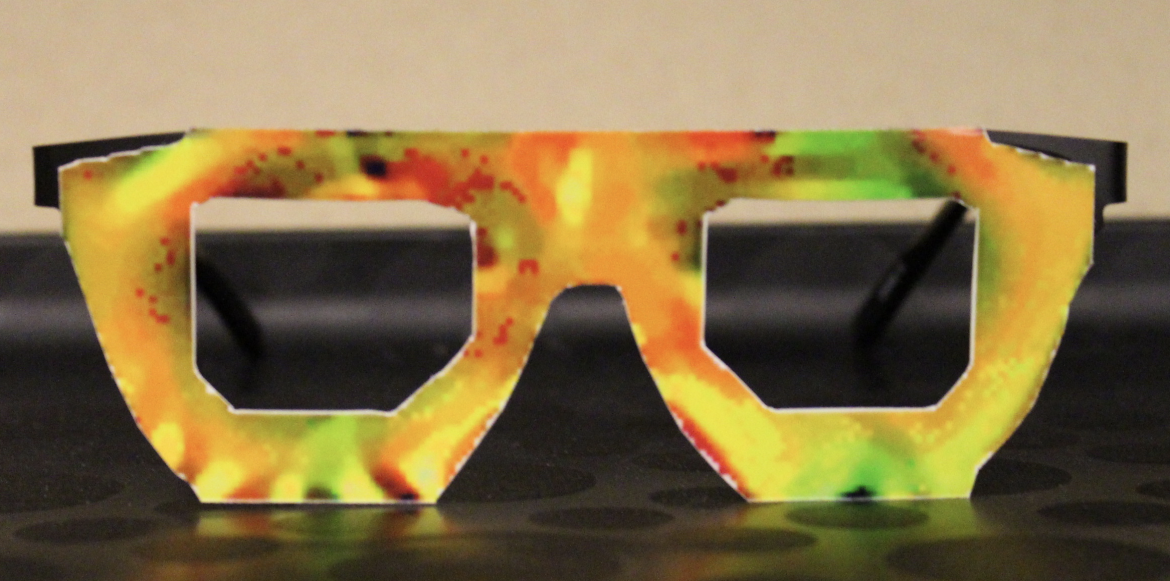
\includegraphics[width=0.4\linewidth]{images/example2.png}
                \caption{Adversarial glasses}
                \label{fig:example2}
            \end{figure}	
        
        \item Shortly after, another research group demonstrated various methods for constructing stop signs that can fool models by placing various stickers on a stop sign. The perturbations were designed to mimic graffiti, and thus “hide in the human psyche.” One of example is showcased in \cref{fig:example3}
        
            \begin{figure}[htbp]
                \centering
                    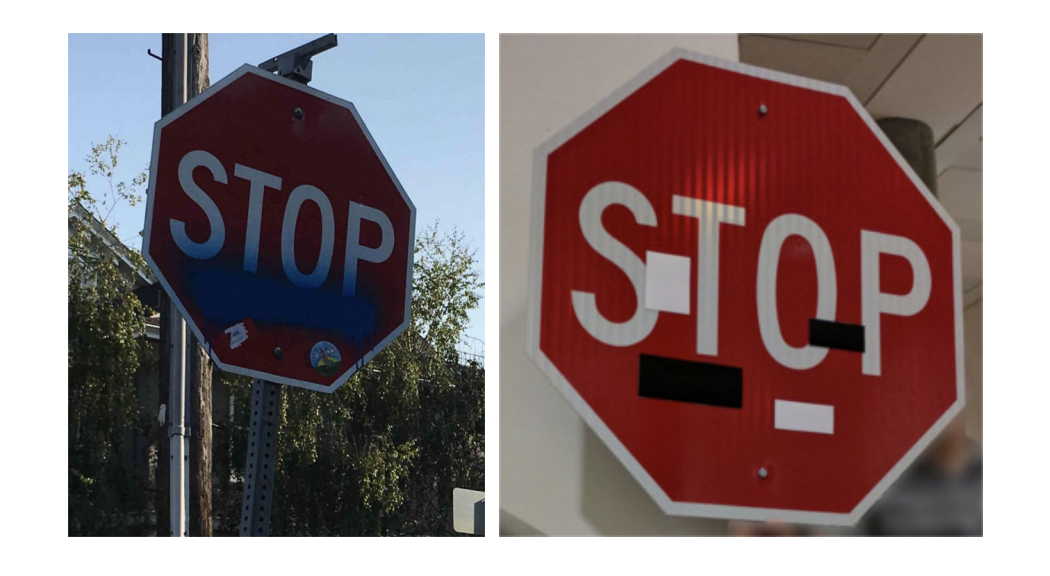
\includegraphics[width=0.4\linewidth]{images/example3.png}
                \caption{Adversarial attack by placing stickers on traffic sign boards}
                \label{fig:example3}
            \end{figure}	
        
        \item “Adversarial Patch”, a paper published at NIPS 2017 demonstrated how to generate a patch that can be placed anywhere within the field of view of the classifier and cause the classifier to output a targeted class. In their experiment, a banana is correctly classified as a banana. They then placed a sticker with a toaster printed on it which is still not enough to fool the network and it still continues to classify it as a banana. However, with a carefully constructed “adversarial patch” by them, they tricked the network into thinking that it’s a toaster. \Cref{fig:example4} represents their experiment. Anyone can download thier paper and print the patch for verification. To quote the authors, “this attack was significant because the attacker does not need to know what image they are attacking when constructing the attack. After generating an adversarial patch, the patch could be widely distributed across the Internet for other attackers to print out and use.”
        
            \begin{figure}[htbp]
                \centering
                    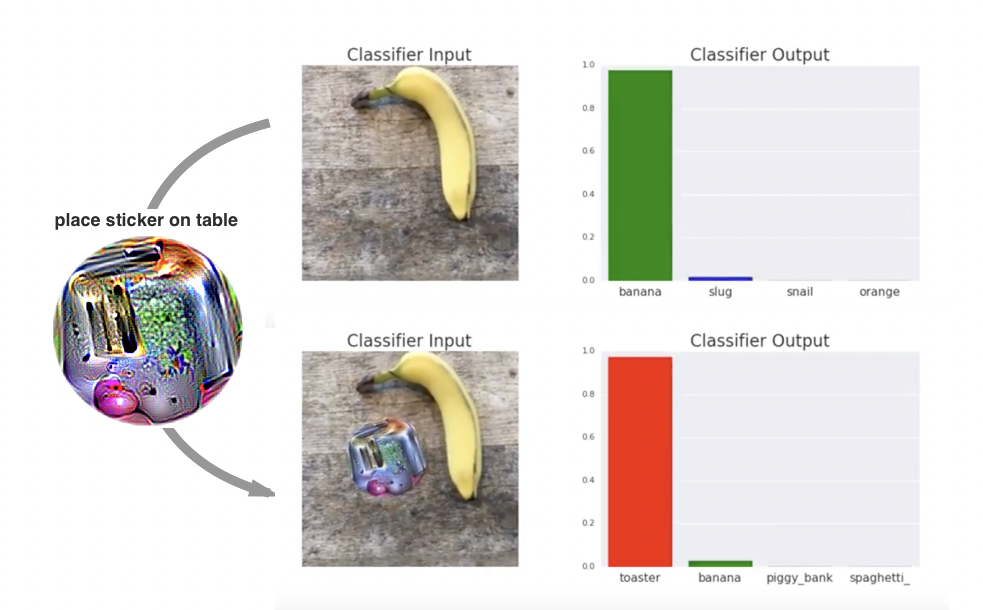
\includegraphics[width=0.7\linewidth]{images/example4.png}
                \caption{An actual image of panda with a perturbation makes a novel deep neural network to misclassify as gibbon.}
                \label{fig:example4}
            \end{figure}	
            
        \item Tesla, an automaker manufactures cars with autopilots. Their autopilots uses a very deep neural network to make decisions. They annualy organises an event and invites attackers to attack their system. Successful attackers gets a price money with gifts. Recently, some researchers performed adversial attack on their deep neural network and made their autopilot to change lane with incoming traffic. They have performed black-box attack. \Cref{fig:example5} give some intuition of the attack performed.
        
            \begin{figure}[htbp]
                \centering
                    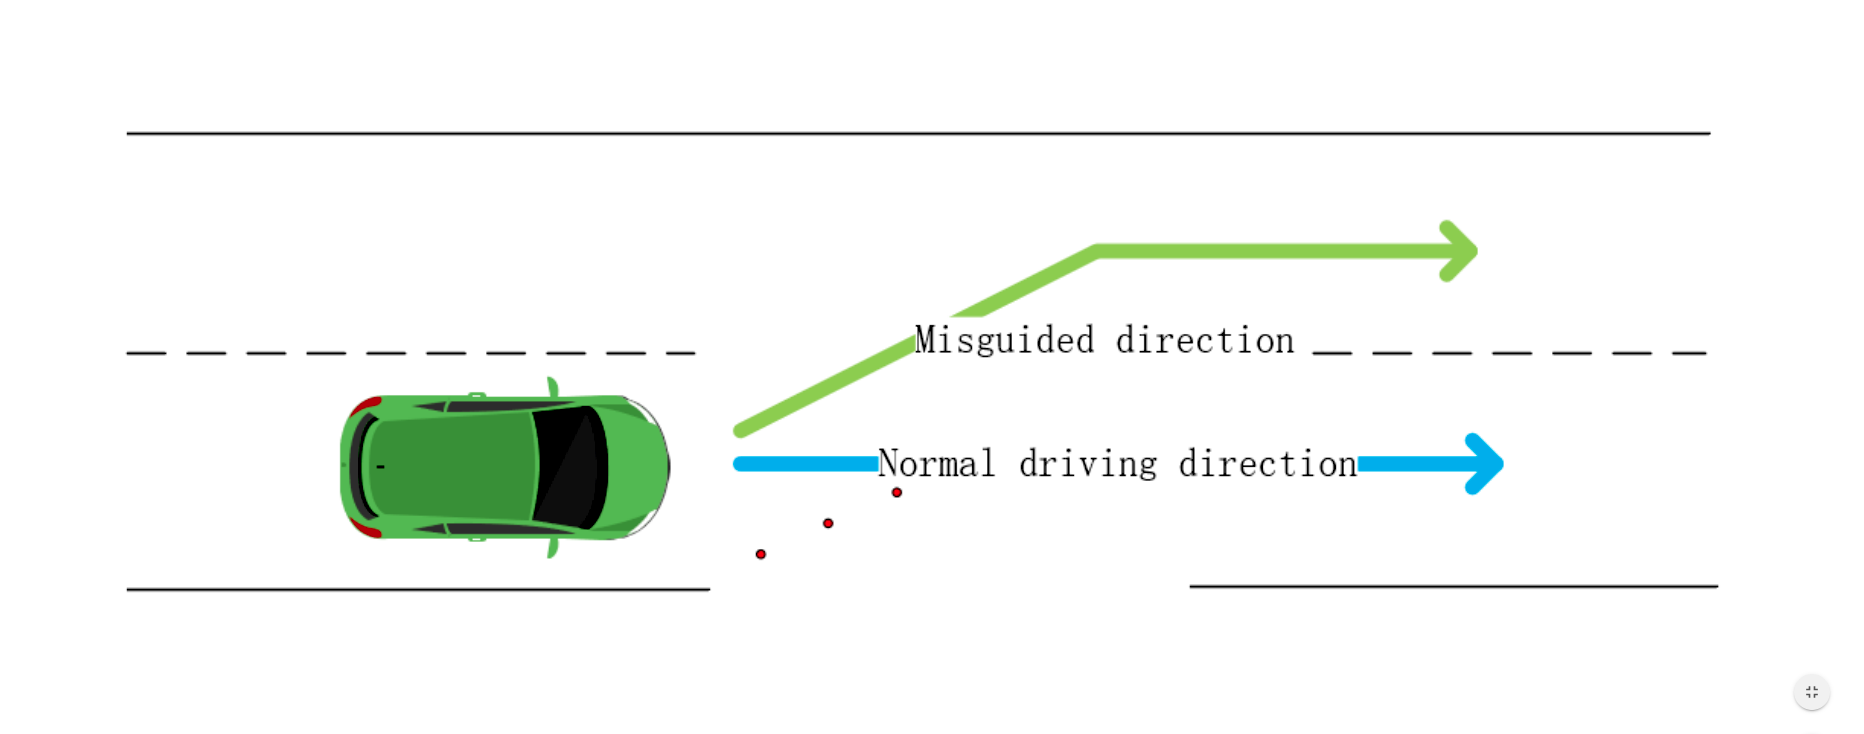
\includegraphics[width=\linewidth]{images/example5.png}
                \caption{An actual image of panda with a perturbation makes a novel deep neural network to misclassify as gibbon.}
                \label{fig:example5}
            \end{figure}
	\end{enumerate}


    % \section{Non-Targeted and Targeted Attacks}

    \subsection{Non-Targeted Attacks}
        The idea is to generate some image that is designed to make the neural network have a certain output. For instance, say our goal label/output is $[0, 0, 0, 0, 0, 1, 0, 0, 0, 0]$.

        That is, we want to come up with an image such that the neural network’s output is the above vector. In other words, find an image such that the neural network thinks the image is a $5$ (remember, we’re zero indexing). It turns out we can formulate this as an optimization problem in much the same way we train a network. Let’s call the image we want to make $\overrightarrow{x}$ (a $784$ dimensional vector, because we flatten out the $28 \times 28$ pixel image to make calculations easier). We’ll define a cost function as $$ C = \frac{1}{2} \Vert y_{goal} - \hat{y}(\overrightarrow{x}) \Vert_{2}^{2} $$

        Where the $y_{goal}$ is our goal label from above. The output of the neural network given our image is $ hat{y}(\overrightarrow{x})$. You can see that if the output of the network given our generated image $\overrightarrow{x}$ is very close to our goal label $ y_{goal}$, then the corresponding cost is low. If the output of the network is very far from our goal then the cost is high. Therefore, finding a vector $\overrightarrow{x}$ that minimizes the cost CC results in an image that the neural network predicts as our goal label. Our problem now is to find this vector $\overrightarrow{x}$. \Cref{fig:non_targeted} shows one of the adversarial image generated by using back propagation with above specified cost function.

        \begin{figure}[htbp]
            \centering
                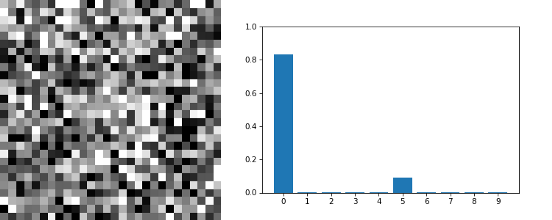
\includegraphics[width=0.7\linewidth]{images/non_targeted1.png}
            \caption{The left side is the non-targeted adversarial exampele (a 28 X 28 pixel image). The right side plots the activations of the network when given the image.}
            \label{fig:non_targeted}
        \end{figure}

    \subsection{Targeted Attacks}
        These adversarial examples are cool and all, but to humans they just look like noise. Wouldn’t it be cool if we could have adversarial examples that actually looked like something? Maybe an image of a $2$ that a neural network thought was a $5$? It turns out that’s possible! And moreover, with just a very small modification to our original code. What we can do is add a term to the cost function that we’re minimizing. Our new cost function will be $$ C = \frac{1}{2} \Vert y_{goal} - \hat{y}(\overrightarrow{x}) \Vert_{2}^{2}  + \lambda \Vert  \overrightarrow{x} - x_{target}  \Vert_{2}^{2}   $$

        Where $x_{target}$ is what we want our adversarial example to look like ($x_{target}$ is therefore a $784$ dimensional vector, the same dimension as our input). So what we’re doing now is we’re simultaneously minimizing two terms. The left term we’ve seen already. Minimizing this will make the neural network output ygoalygoal when given $(\overrightarrow{x}$. Minimizing the second term will try to force our adversarial image x to be as close as possible to $x_{target}$ as possible (because the norm is smaller when the two vectors are closer), which is what we want! The extra $\lambda$ out front is a hyperparameter that dictates which of the terms is more important. As with most hyperparameters I find after a lot of trial and error that $.05$ is a good number to set $\lambda$ to. If you know about ridge regularization you might find the cost function above very very familiar. In fact, we can interpret the above cost function as placing a prior on our model for our adversarial examples.

    \subsection{Performing a Targeted Attack} \label{sec:targetedattack}
        This subsection describes the steps taken to perform a targeted adversarial attack. on a trained neural network. This is a white box attack, in which I have full information about the network use, it's parameters and it's structure. This section describes steps taken to perform the attack. Source code is available on Github (https://github.com/rishitoshsingh/Adversarial-Attack). 

        \begin{enumerate}
            \item \textbf{Choosing dataset - MNIST}

                \begin{figure}[b]
                    \centering
                    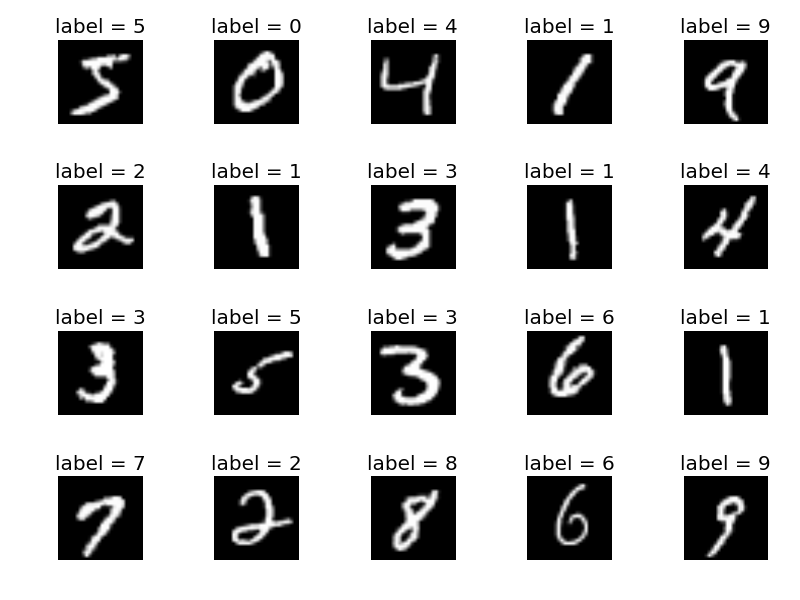
\includegraphics[width=0.5\linewidth]{images/mnist.png}
                    \caption{Some samples of MNIST dataset}
                    \label{fig:mnist}
                \end{figure}
                    
                The MNIST database (Modified National Institute of Standards and Technology database) is a large database of handwritten digits that is commonly used for training various image processing systems. The database is also widely used for training and testing in the field of machine learning. It was created by "re-mixing" the samples from NIST's original datasets. The creators felt that since NIST's training dataset was taken from American Census Bureau employees, while the testing dataset was taken from American high school students, it was not well-suited for machine learning experiments. Furthermore, the black and white images from NIST were normalized to fit into a $28 \times 28$ pixel bounding box and anti-aliased, which introduced grayscale levels. I have used $10\%$ of this dataset due to limitation of computation power and time.

            \item \textbf{Training neural network}

                Next step is to train a neural network on whom white-box attack is to be performed. I have trained a neural network with one hidden layer having $20$ neurons and one output layer having $10$ neurons. So the structure of network is $784 - [20] - 10$. The trained network performs well in test dataset. 	

            \item \textbf{Generating adversarial image}

                In this step we will use back propagation with modified error function on already trained neural network. During this process, neural network's weights are not learnable parameters, but inputs are learnable. At the beginning a random sample from dataset is fed to trained neural network. At each iteration, algorithm make relevant modifications to this input such that network make misclassification with less visual modifications on actual image.

        \end{enumerate}

    \subsection{Generated adversarial images and results}

        \Cref{fig:generated} shows some of the generated adversarial images using steps mentioned is \cref{sec:targetedattack}. All but one generated images were clearly successful in fooling trained neural network. \Cref{fig:generated} (\subref{fig:sfig4}) shows a random sample of $6$ digit with it's corresponding generated adversarial image. The trained neural network was $89\%$ confident that figure in right is $6$, but the network is $37\%$ confident that image in left is $6$. The confidence of network decreases in case of adversarial image, thus it can be concluded that all of the shown images were successful in fooling a trained neural network. 

        \begin{figure}[htbp]
            \begin{subfigure}{.5\textwidth}
                \centering
                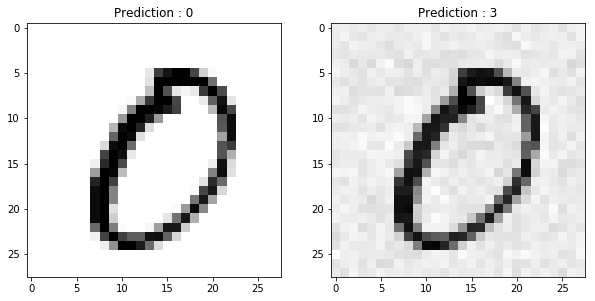
\includegraphics[width=\linewidth]{images/adversarial1.png}
                \caption{ }
                \label{fig:sfig1}
            \end{subfigure}
            \begin{subfigure}{.5\textwidth}
                \centering
                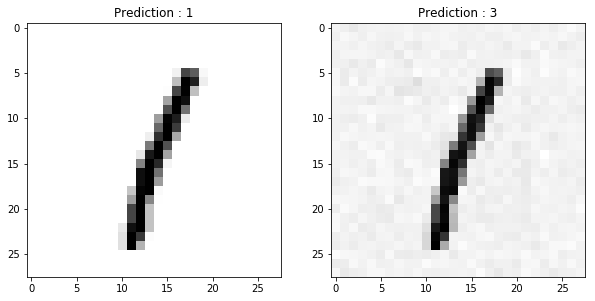
\includegraphics[width=\linewidth]{images/adversarial2.png}
                \caption{ }
                \label{fig:sfig2}
            \end{subfigure}
            \begin{subfigure}{.5\textwidth}
                \centering
                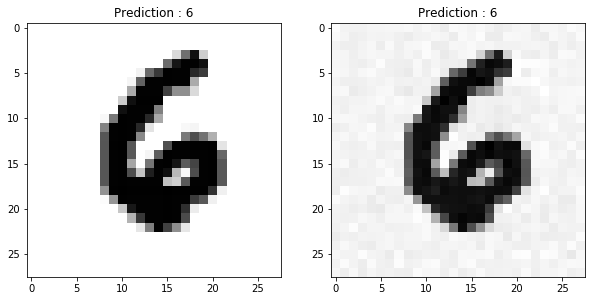
\includegraphics[width=\linewidth]{images/adversarial3.png}
                \caption{ }
                \label{fig:sfig3}
            \end{subfigure}
            \begin{subfigure}{.5\textwidth}
                \centering
                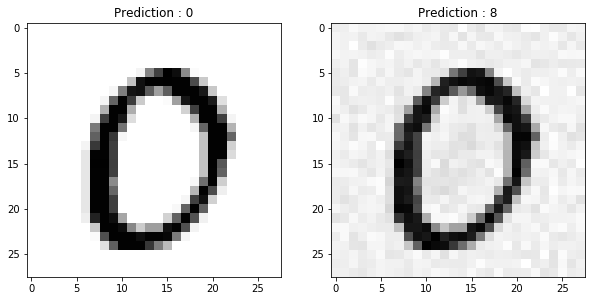
\includegraphics[width=\linewidth]{images/adversarial4.png}
                \caption{ }
                \label{fig:sfig4}
            \end{subfigure}
            \caption{Left side image is actual image from dataset and right side image is generated adversarial image}
            \label{fig:generated}
        \end{figure}


    % \section{Protecting Against Adversarial Attacks}

    \subsection{Binary Thresholding}

        We’ve just created images that trick neural networks. The next question we could ask is whether or not we could protect against these kinds of attacks. If you look closely at the original images and the adversarial examples you’ll see that the adversarial examples have some sort of grey tinged background.

        \begin{figure}[htbp]
            \centering
            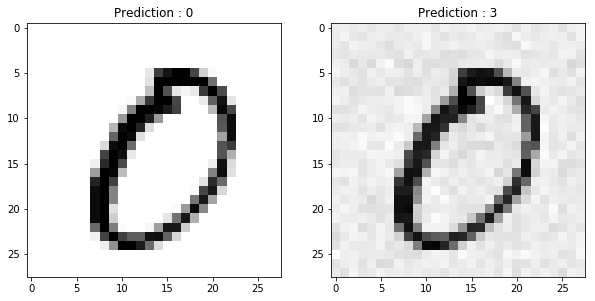
\includegraphics[width=0.7\linewidth]{images/adversarial1.png}
            \caption{Generated Adversarial Image}
        \end{figure}

        \begin{figure}[htbp]
            \centering
            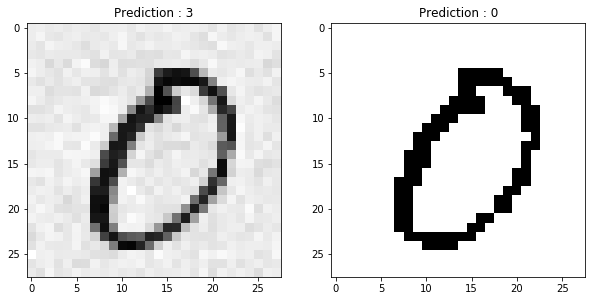
\includegraphics[width=0.7\linewidth]{images/thresholding.png}
            \caption{The effect of binary thresholding on an MNIST adversarial image. The left image is the adversarial image, the right side is the binarized image}
        \end{figure}

        One naive thing we could try is to use binary thresholding to completely white out the background. Turns out binary thresholding works! But this way of protecting against adversarial attacks is not very good. Not all images will always have an all white background. For example in \cref{fig:panda_thresholding},	 panda at the very beginning of this post. Doing binary thresholding on that image might remove the noise, but not without disturbing the image of the panda a ton. Probably to the point where the network (and humans) can’t even tell it’s a panda.
                
        \begin{figure}[htbp]
            \centering
            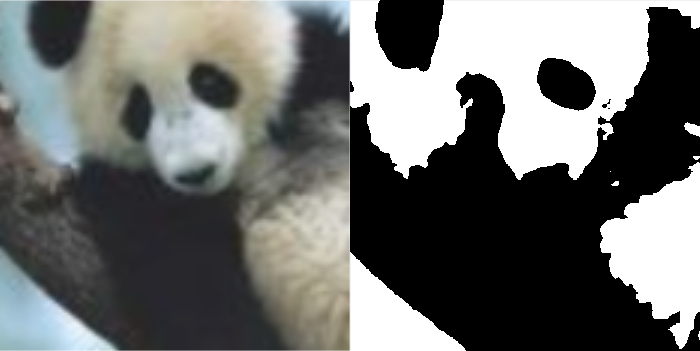
\includegraphics[width=0.7\linewidth]{images/panda_thresholding.png}
            \caption{Doing binary thresholding on the panda results in a blobby image}
            \label{fig:panda_thresholding}
        \end{figure}

    \subsection{Adversarial training}
        One of the easiest and most brute-force way to defend against these attacks is to pretend to be the attacker, generate a number of adversarial examples against your own network, and then explicitly train the model to not be fooled by them. This improves the generalization of the model but hasn’t been able to provide a meaningful level of robustness — in fact, it just ends up being a game of whack-a-mole where attackers and defenders are just trying to one-up each other.

    \subsection{Defensive distillation}
        In defensive distillation, we train a secondary model whose surface is smoothed in the directions an attacker will typically try to exploit, making it difficult for them to discover adversarial input tweaks that lead to incorrect categorization. The reason it works is that unlike the first model, the second model is trained on the primary model’s “soft” probability outputs, rather than the “hard” (0/1) true labels from the real training data. This technique was shown to have some success defending initial variants of adversarial attacks but has been beaten by more recent ones, like the Carlini-Wagner attack, which is the current benchmark for evaluating the robustness of a neural network against adversarial attacks.

    \subsection{Why is defending neural networks so hard?}
        Let’s try to develop an intuition behind what’s going on here. Most of the time, machine learning models work very well but only work on a very small amount of all the many possible inputs they might encounter. In a high-dimensional space, a very small perturbation in each individual input pixel can be enough to cause a dramatic change in the dot products down the neural network. So, it’s very easy to nudge the input image to a point in high-dimensional space that our networks have never seen before. This is a key point to keep in mind: the high dimensional spaces are so sparse that most of our training data is concentrated in a very small region known as the manifold. Although our neural networks are nonlinear by definition, the most common activation function we use to train them, the Rectifier Linear Unit, or ReLu, is linear for inputs greater than $0$.

        \begin{figure}[htbp]
            \centering
            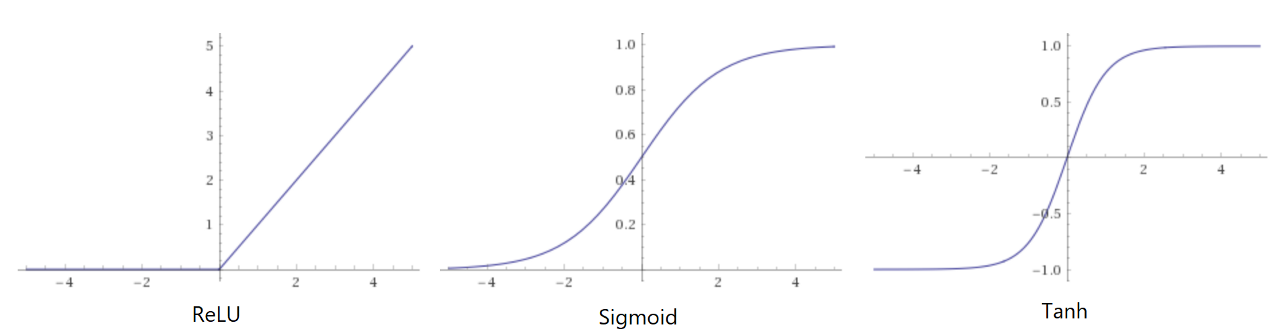
\includegraphics[width=\linewidth]{images/functions.png}
            \caption{The Rectifier Linear Unit, or the ReLu compared to the Sigmoid and the Tanh activation functions.}
        \end{figure}

        ReLu became the preferred activations function due to its ease of trainability. Compared to sigmoid or tanh activation functions that simply saturate to a capped value at high activations and thus have gradients getting “stuck” very close to $0$, the ReLu has a non-zero gradient everywhere to the right of $0$, making it much more stable and faster to train. But, that also makes it possible to push the ReLu activation function to arbitrarily high values.

        Looking at this trade-off between trainability and robustness to adversarial attacks, we can conclude that the neural network models we have been using are intrinsically flawed. Ease of optimization has come at the cost of models that are easily misled.		


    % \section{Conclusion}

    In this paper, a gradient-based adversarial image generation algorithm is proposed. Using the proposed algorithm, the adversary can generate adversarial images for target and non-target adversarial attacks. Neural networks are a black box, what a network learns is still unknown, which makes them more vulnerable to be duped. This paper demonstrated that tricking neural networks using adversarial examples is an easy task. Just like an ANN, all complex neural networks such as CNN are also susceptive to adversarial attacks. Instead of employing neural networks in every possible scenario, a tremendous amount of research is required to protect them from these attacks. 
    

    \crefname{appsec}{Appendix}{Appendices}

\appendixtitleon
\begin{appendices}
    \setcounter{equation}{0}
    \numberwithin{equation}{section}

    \crefalias{section}{appsec}

    \section*{Derivation of learning rules}\label{apendix:derivation_of_learning_rule} 

        Consider a trained three-layered neural network with structure $(L-M-N)$ consisting of $L$ inputs, $M$ hidden neurons, and $N$ output neurons. The output of $m^{th}$ neuron $Y_m$ is computed by activation function of net potential ($V_m$), where $V_m$ and $Y_m$ are defined respectively as
        \begin{align} \label{eqn:Vm}
            V_m =  \sum \limits_{l=1}^{L} w_{lm}x_{l} + w_{0m}x^{0}
        \end{align} and	
        \begin{align}\label{eqn:Ym}	
            Y_m =&\quad f(V_m)
        \end{align}
        Similarly, the respective net potential ($V_n$) and output ($Y_n$) of $n^{th}$ output neuron are given as
        \begin{align}\label{eqn:Vn}
            V_n =\sum \limits_{m=1}^{M} w_{mn}Y_{m} + w_{0n}x^{0} 
        \end{align} and 
        \begin{align} \label{eqn:Yn}
            Y_n =& \quad f(V_n)  
        \end{align}
        Let $Y_n^{Adv}$ be the desired adversary output at $n^{th}$ neuron, then the error, $e_n^Y$ at $n^{th}$ output neuron is calculated through the difference between $Y_n$ and $Y_n^{Adv}$, which is expressed as
        \begin{align} \label{eqn:eny} 
            e_n^Y =& Y_n^D - Y_n
        \end{align} 
        and let $x^{Adv}$ be the desired adversarial image, then the error $e_l^x$ at $l^{th}$ input is calculated through the difference between $x_l$ and $x_l^{Adv}$, which is expressed as
        \begin{align} \label{eqn:enx} 
            e_l^x =& x_l^{Adv} - x_l
        \end{align} 
        The cost function $E$ (MSE) can be calculated by
        \begin{align} \label{eqn:mse}
            E =& \quad \frac{1}{2N} \sum \limits_{n=1}^{N} (e_n^Y)^{2} + \lambda \frac{1}{2L} \sum \limits_{l=1}^{L} (e_l^x)^{2}
        \end{align}
         
        During adversarial image generation, inputs are adaptable instead of network weights. The gradient-decent based backpropagation is used to minimize the cost function. The current input $x^{old}$ is updated to $x^{new}$ using $\Delta x$ as 
        \begin{align} \label{eqn:update_rule}
            x^{old} = x^{new} + \Delta x
        \end{align}
        where $\Delta x$ is promotional to negative gradient of cost function $(\nabla_{x}E)$.
        \begin{align} \label{eqn:delta_x}
            \Delta x &= - \eta \nabla_{x} E \nonumber \\ 
                     &= - \eta \cdot \frac{\partial E}{\partial x}
        \end{align}
        For input $x_{l}$, $- \partial E / \partial x_{l}$ is derived using chain rule of derivation.
        \begin{align} \label{eqn:delta_e_x}
            - \frac{\partial E }{\partial x_{l}} = \frac{1}{N} \sum \limits_{n=0}^{N} \left\{ e_n^Y \cdot f'(V_n) \cdot \frac{\partial V_n}{\partial x_l} \right\} + \frac{\lambda}{L} e_l^x
        \end{align}
        Now, substituting \cref{eqn:delta_e_x} in \cref{eqn:delta_x} yields 
        \begin{align} \label{eqn:delta_x_2}
            \Delta x_l  = \frac{\eta}{N} \left\{ \sum \limits_{n=0}^{N} \delta_{n} w_{mn} \right\} \nabla_{x_l} Y_m + \lambda \frac{\eta}{L} e_l^x
        \end{align}
        where $\delta_{n} = e_n^Y f'(V_n)$

        Now using \cref{eqn:Ym,eqn:Vm}, $\nabla_{x_l} Y_m$ can further be simplified using chain rule of derivation
        \begin{align} \label{eqn:nabla_vn}
            \nabla_{x_l} Y_m &= \sum \limits_{m=0}^{M} \left\{ f'(V_m) \frac{\partial V_m}{\partial x_l} \right\} \nonumber \\
            &= \sum \limits_{m=0}^{M} f'(V_m) w_{lm}
        \end{align}
        
        Now, substituting \cref{eqn:nabla_vn} in \cref{eqn:delta_x_2} yields

        \begin{align} \label{eqn:final_learning_eqn}
            \Delta x= \frac{\eta}{N} \sum \limits_{m=0}^{M} \delta_{m} w_{lm} + \lambda \frac{\eta}{L} e_l^x
        \end{align}
        where,
        \begin{align}
            \delta_{m} = \left\{ \sum \limits_{n=0}^{N} \delta_{n} w_{mn} \right\} f'(V_m) \nonumber
        \end{align}      

\end{appendices}

    \bibliography{mybib}{}
    \bibliographystyle{plain}
\end{document}